\documentclass[11pt]{article}
\usepackage[utf8]{inputenc}
\usepackage[spanish, mexico]{babel}
\usepackage{listings}
\usepackage{breakcites}
\usepackage{dsfont}
\usepackage{hyperref}
\usepackage{amssymb,amsthm,amsmath,latexsym}
\usepackage[margin=1.5cm]{geometry}
\usepackage{natbib}
%\bibliographystyle{stylename}
%\usepackage{fancyhdr}
%\pagestyle{fancy}
\theoremstyle{plain}
\newtheorem{teo}{Teorema}
\newtheorem{prop}[teo]{Proposición}
\newtheorem{defi}[teo]{Definición}
\newtheorem{obs}[teo]{Observación}
\newtheorem{lem}[teo]{Lema}
\newtheorem{cor}[teo]{Corolario}
\usepackage[pdftex]{color,graphicx}
\newcommand{\sgn}{\mathop{\mathrm{sgn}}}
\title{Survey}
\author{Mauricio Gonzalez Soto}
\begin{document}
\nocite{*}
\maketitle
\tableofcontents
\newpage
\section{Introducción}
El problema que estamos tratando de atacar consiste en descubrir relaciones causales que se encuentren presentes en diversos fenómenos. El enfoque que se propone es descubrir estas relaciones mediante \textit{interacción} con el entorno. En el contexto de inferencia causal, los datos que, usualmente, se tienen provienen de fuentes ruidosas por lo que la probabilidad será el lenguaje adecuado para razonar sobre estos datos.\\
\\
\cite{lake2017building} argumentan que los sistemas inteligentes actuales, a pesar de sus impresionantes logros, aun están lejos de alcanzar una verdadera inteligencia; uno de los requisitos para esto es que puedan construir modelos causales que sean interpretables, y no sólo reconocer patrones estadísticos. 
\\
La primera parte de este resumen consiste en el estudio clásico de relaciones causales, el cual depende fuertemente de Redes Bayesianas, las cualesson objetos matemáticos utilizados para representar distribuciones de probabilidad de manera eficiente; además, permiten incorporar conocimiento inicial sobre las variables aleatorias representadas en la red. Debido a que estas redes son de fácil interpretación, es natural definir modelos causales en términos de estas, pues fácilmente nodos y aristas pueden traducirse en términos de objetos y causas.\\
\\
Después, veremos que existe un área del aprendizaje de máquina llamado Aprendizaje por Refuerzo, que es un marco teórico para el aprendizaje automático en el cual un \textit{agente} aprende a realizar una tarea a través de experiencia y de interacción con su entorno.\\
\\
Además, las intuiciones iniciales sobre aprendizaje causal por interacción provienen de estudios realizados en Psicología Computacional y Ciencias Cognitivas, de aquí se sabe que los seres humanos obtienen conocimiento causal al encontrarse en situaciones en las cuales deben tomar decisiones de manera secuencial para lograr un objetivo futuro. Se sabe también que el conocimiento causal adquirido puede ser utilizado para mejorar las futuras decisiones tomadas.\\
\\
Notando que los modelos causales tradicionales requieren de intervenciones y experimentación en el mundo, y que estas intervenciones son una forma de interacción y alteración del mundo, salta a la vista la relación entre Aprendizaje por Refuerzo y aprendizaje causal. Entonces, resulta natural preguntar cómo pueden aprenderse relaciones causales de manera interactiva de modo que el conocimiento causal adquirido permita a un agente tomar mejores decisiones. La pregunta se convierte entonces en cómo obtener e incorporar conocimiento causal en un problema de aprendizaje por refuerzo. Además, uno se pregunta si es posible utilizar este conocimiento causal obtenido al interactuar sobre el mundo para realizar otro tipo de inferencias causales en ciertos dominios de interés.
\section{Causalidad}
\subsection{Intro}
Saber si es posible hablar de relaciones causa-efecto es un tema polémico; los métodos probabilistas tradicionales sólo codifican asociaciones estadísticas, pero la idea
La diferencia entre modelos probabilistas y modelos causales se da cuando es de interés tomar acciones que modifiquen el entorno y no nada más observar los valores de las variables. \\
Según \cite{pearl2014probabilistic}, las dos preguntas fundamentales en Causalidad son:
\begin{itemize}
\item ¿Qué evidencia empírica es necesaria para hacer inferencias válidas sobre relaciones causa-efecto?
\item Dado que estamos dispuestos a aceptar información causal sobre un fenómeno, ¿qué inferencias podemos obtener a partir de esta información, y cómo?
\end{itemize}
En cuanto al segundo punto, Pearl considera que hay tres tipos de preguntas a considerar
\begin{itemize}
\item Predicciones: si sabemos que una persona ingirió alimentos de dudosa procedencia, ¿se enfermará?
\item Intervenciones: si le damos cierto tratamiento a un paciente, ¿mejorará?
\item Contrafactuales: ¿el paciente del punto uno se habría enfermado de todos modos si no hubiera consumido esos alimentos?
\end{itemize}
Pearl argumenta que aunque causalidad suele entenderse como afirmaciones necesarias, estas son hechas en contexto de incertidumbre, por lo que cualquier teoría causal debe estar en términos de probabilidades.
\subsection{Un poco de historia}
Aristóteles definió 4 \textit{causas} para una cosa, una de ellas llamada \textit{causa eficiente} que estaba definida como aquello que hace la cosa.\\
\\
En 1690, el filósofo inglés John Locke propuso como definición de causa “aquello que produce alguna idea simple o compleja”, y lo que es producido lo definió como efecto.\\
\\
\cite{holland1986statistics} resalta la importante diferencia en que Aristóteles hizo énfasis en las causas de una cosa, pero no en el efecto de estas. \\
\\
Fue David Hume quien se considera que hiz una importante contribución, y él definió la causalidad como una relación entre experiencias más que una entre hechos. Argumentó que no es verificable empíricamente que la causa produzca el efecto, sino sólo que el evento llamado \textit{causa} es invariablemente seguido por aquella experiencia llamada \textit{efecto}.\\
\\
Hume definió 3 criterios básicos para causalidad:
\begin{itemize}
\item Contiguidad espacio-temporal: tanto causa y efecto tienen lugar en una entidad común (espacio y tiempo).
\item Sucesión temporal: La causa tiene que preceder temporalmente al efecto. 
\item Conjunción constante: Causa y efecto ocurren juntos, o no ocurren juntos.
\end{itemize}
John Stuart Mill argumentó tajantemente que observación sin experimentos no puede probar causalidad. Mill identificó cuatro métodos generales para la identificación de relaciones causales. 
\subsection{Modelo de Rubin}
El modelo de Rubin parte de una población de \textit{unidades} $U$. En general, estas unidades son los objetos de estudio sobre las cuales actuan las causas. Para hacer más sencilla la descripción del modelo, supondremos que sólo existen dos causas (o niveles de tratamiento) denotadas por $t$ y $c$. Sea $S$ una variable indicadora de la causa a la cual cada unidad $u \in U$ fue expuesta. Además, consideramos dos variables respuesta $Y_t$, $Y_c$. $Y_t(u)$ reoresenta el valor de la respuesta si la unidad $u$ es expuesta a $t$ y análogo para $c$.\\
\\
\begin{defi}
Se define el efecto de la causa $t$ sobre $u$ relativo a la causa $c$ como
\[ Y_t(u) - Y_c(u). \]
Esta expresión se lee de la siguiente manera: $t$ causa el efecto $Y_t(u) - Y_c(u)$ en la unidad $u$ (relativo al control $c$).
\end{defi}
Notemos que es imposible observar simultáneamente el efecto de $t$ y de $c$ sobre una misma unidad $u$ y a esto \cite{holland1986statistics} le llama el Problema Fundamental de la Inferencia Causal. El problema, según explica Holland, radica en la palabra \textit{observar} pues no podemos saber simultáneamente el efecto de exponer a un enfermo en particular a un nuevo tratamiento y al mismo tiempo el efecto de no exponerlo.
\subsection{Modelo de Suppes}
En su libro “Probabilistic Theory of Causality”, (\cite{suppes1970probabilistic}), Patrick Suppes intenta mejorar el análisis de Hume sobre causalidad; en particular, la condición de conjunción constante. Para Suppes, no importa qué sean las causas y los efectos, sino que se puedan expresar como eventos que ocurren bajo ciertas condiciones. Suppes supone que todas las causas necesariamente preceden en el tiempo a sus efectos. Define una causa \textit{prima facie} de un evento como un evento que precede temporalemnte a este y que está asociado de manera positiva con él. Define como una causa espuria a una causa prima facie tal que es condicionalmente independiente del efecto dada otra causa la cual es anterior en el tiempo a la causa prima facie y que está asociada con el evento dada la causa. Una causa genuina es una causa prima facie que no es espuria.
\begin{defi}
Si $r < s$ representan valores de tiempo, se dice que el evento $C_r$ es una causa prima facie del evento $E_s$ si
\[ P(E_s | C_r ) > P(E_s). \]
\end{defi}
\begin{defi}
Un evento $C_r$ se dice que es una causa espuria de un eventi $E_s$ si $C_r$ es una causa prima facie de él y para alguna $q < r < s$ existe un evento $D_q$ tal que 
\[P(E_s | C_r, D_q) = P (E_s | D_q) \]
y además,
\[P(E_s | C_r , D_q) \geq P(E_s | C_r). \]
\end{defi}
Por lo tanto,
\begin{defi}
Para tiempos $r < s$, un evento $C_r$ se dice que es una causa genuina de un evento $E_s$ si $C_r$ es una causa prima facie de $E_s$, pero no es una causa espuria.
\end{defi}
Notemos que Suppes está definiendo la causa de un efecto, más que el efecto de una causa. Además, no hay restricciones a la naturaleza de una causa más allá de que sea un evento que ocurre antes en el tiempo. El modelo de Suppes no puede expresar el efecto de una causa en particular, sólo comportamientos promedio (\cite{holland1986statistics}).\\
\\
En palabras de Holland, la causalidad de Suppes no es más que correlación entre causa y efecto que no puede ser eliminada al parcializar causas legítimas.
\subsection{Modelos Causales en Medicina}
Un caso de aplicación en medicina es determinar que ciertas bacterias causan ciertas enfermedades. Existe un conjunto de postulados planteados por Koch para decidir cuándo un micro-organismo está implicado en una enfermedad. Aunque no existe un planteamiento formal, estos pueden expresarse como (\cite{yerushalmy1959methodology}):
\begin{itemize}
\item El organismo debe estar presente en todos los casos de la enfermedad supuestamente provocada por él.
\item El organismo debe aislarse de los pacientes y cultivarse en estado puro.
\item El organismo cultivado en estado puro debe reproducir el padecimiento. 
\end{itemize}
Estos postulados aseguran que no haya datos que apoyen una hipótesis nula de cero efecto causal. \\
\\
Por otro lado, Hill, quien fue de los primeros en estudiar la asociación entre fumar y cáncer, encontró 9 factores útiles a la hora de decidir que una asociación observada es causal. 
\subsection{Causalidad de Granger en Economía}
La causalidad de Granger se utiliza para series de tiempo, lo cual es de alta importancia en Economía. \cite{holland1986statistics} opina que las ideas esenciales de Granger no están limitadas a series de tiempo y que pueden ser expresadas en términos de variables que actuan sobre unidades de una población.\\
\\
En la teoría de Granger, una variable causa otra variable; es decir ( \cite{holland1986statistics}), las realizaciones de una variable mejoran las predicciones hechas sobre la otra variable. La única parte en la que se utilizan series de tiempo en esta definición es para hablar de valores de las variables definidos hasta un cierto tiempo $t$.\\
\\
Si $X,Y,Z$ son variables aleatorias definidas sobre cierta población, se dice que $X$ no es una causa de Granger de $Y$ si $X$ y $Y$ son condicionalmente independientes dado $Z$. Entonces, $X$ es una causa de Granger de $Y$ si distintos valores de $X$ llevan a distintas distribuciones predictivas de $Y$ dados $X$ y $Z$; esto es, $X$ ayuda a predecir $Y$ aun cuando $Z$ es tomada en cuenta. La no-causalidad de Granger es parecida a las causas espurias de Suppes pues ambas consideran que no se pueda predecir un evento dada cierta información.\\
\\
En opinión de Holland, la causalidad de Granger falla de la misma manera que la de Suppes, pues a la luz de nueva información una causa Granger puede dejar de serlo.
\subsection{Modelos Causales en Ciencias Sociales}
\subsection{Aprendizaje de Modelos Causales a partir de datos}
En los métodos de estado del arte de Modelos Causales Funcionales suele hacerse los siguientes supuestos (\cite{goudet2017learning}):
\begin{itemize}
\item Suficiencia Causal (CSA)
\item Propiedad Markoviana (CMA)
\item Independencias Condicionales
\item Fiabilidad causal (CFA)
\end{itemize}
\subsubsection{Aprender el CPDAG}
Existen tres familias de métodos para extraer el grafo: métodos de restricciones, métodos de score y métodos híbridos.\\
\\
Los métodos basados en restricciones explotan las independencias condicionaes para identificar todas las v-estructuras. El algoritmo más conocido es el Algoritmo PC (\cite{spirtes2000causation}). El algoritmo PC primero construye un esqueleto basado en independencias condicionales; luego, identifica las v-estructuras y posteriormente orienta las aristas. El algoritmo FCI (\cite{spirtes1999algorithm}) extiende el algoritmo PC al relajar la suficiencia causal e incorporar variables latentes. El algoritmo RFCI de \cite{colombo2012learning} es más rápido que FCI y maneja datos de alta dimensionalidad. La debilidad de estos métodos, según \cite{goudet2017learning} es que dependen demasiado en pruebas de independencia, que dependen a su vez de la cantidad disponible de datos.\\
\\
Los métodos basados en score exploran el espacio de CPDAG's y minimizan un score global. La exploración se realiza en términos de operaciones sobre grafos, por ejemplo añadir o remover aristas. El algoritmo Greedy Equivalent Search (GES) de \cite{chickering2002optimal} encuentra la estructura óptima en términos del BIC.\\
\\
Los métodos híbridos combinan las técnicas anteriores. Por ejemplo el Max-Min Hill Climbing Algorithm de \cite{tsamardinos2006max} primero construye un esqueleto utilizando pruebas de independencia condicional, y luego le da orientación a las aristas utilizando un método greedy sobre un score bayesiano.
\subsubsection{Explotando la asimetría entre causa y efecto}
Los métodos anteriores no toman en cuenta la asimetría entre causas y efectos. La intuición detrás (\cite{goudet2017learning}) está dada por el siguiente ejemplo: Si consideramos el modelo causal funcional $Y=X+U$, entonces los métodos anteriores basados en grafos no pueden darle orientación a la arista $X - Y$, pues tanto $X \rightarrow Y$ como $Y \rightarrow X$ son Markov equivalentes.\\
\\
\cite{stegle2010probabilistic} infiere la dirección causal al construir dos modelos Bayesianos generativos: uno para $X \rightarrow Y$ y otro para $Y \rightarrow X$. La dirección causal es determinada a partir del modelo generativo que mejor ajuste a los datos. Otros métodos, como el propuesto por \cite{sgouritsa2015inference} se basan en que si $X \rightarrow Y$, entonces la probabilidad marginal de la causa $P(X)$ es independiente del mecanismo causal $P(X | Y)$; por lo tanto, estimar $P(Y | X)$ a partir de $P(X)$ no debería poderse, pero estimar $P(X | Y)$ a partir de $P(Y)$ sí debería ser posible.
\subsubsection{Como problema de Aprendizaje}
Inspirados en los concursos de Kaggle de \cite{Guyon2013}, \cite{lopez2015towards} plantean el problema de inferencia causal como un problema de clasificación de medidas de probabilidad. Los datos provistos por el concurso son 16,200 parejas de variables $(X_i,Y_i)$. Cada par consta de una realización $(x_i,y_i)$ y una etiqueta $l_i$ que indica el valor de la verdadera relación causal; es decir, $l_i$ indica uno de los siguientes casos: $X \rightarrow Y,$ $Y \rightarrow X$, $X_i \perp Y_i$, $X \leftrightarrow Y$.\\
\\
Notemos que este método tiene como punto débil que depende de la representatividad de la muestra de entrenamiento y que supone la existencia de una distribución madre
\subsubsection{Modelos Causales Funcionales Neuronales}
\cite{goudet2017learning} proponen un esquema que consiste en tres pasos: primero, identificar el esqueleto según propiedades de independencia estándar; luego, orientar las aristas utilizando métodos bivariados estándar y finalmente hacer una optimización sobre todo el grafo examinando relaciones locales. Este último paso se realiza al aprender estos modelos locales como redes neuronales generativas; es decir, se modela la distribución $P(X | X_{Pa_i}, U_i)$ de un nodo condicional en sus padres (causas) con una red neuronal.\\
\\
Formalmente, se modela cada ecuación
\[X_i = f_i (X_{Pa_i},U_i) \]
como una red neuronal generativa global, en la cual cada función $f_i$ es modelada por una red neuronal generativa con una capa oculta.\\
\\
Encontrar un modelo causal de este tipo requiere llevar a cabo dos tareas: estimar la estructura (el grafo) de los padres de cada variable, y las redes neuronales $f$
\subsection{Correlación y causalidad}
Dos variables aleatorias $X$,$Y$ pueden estar correlacionadas en distintos casos; por ejemplo, si $X$ causa $Y$, o si tanto $X$ como $Y$ son causadas por otra variable desconocida $V$. Si e conoce la existencia de $V$ y además podemos observarla. 

\section{Modelos Gráficos Probabilistas}

\section{Modelos gráficos causales}
Sabemos que en una red bayesiana los arcos, aunque dirigidos, no necesariamente tienen una interpretación directa, lo único que importa es que el grafo capture adecuadamente las relaciones de dependencia entre variables aleatorias. Nos gustaría que fuera el caso que $X \to Y$ significara $X$ \textit{causa} Y. Resulta que existe una familia de modelos causales en los cuales se \textit{interviene} en el mundo. La idea clave es utilizar \textit{intervenciones ideales}, las cuales se denotan $do(Z=z)$ que significa forzar a la variable aleatoria $Z$ a tomar el valor $z$, denotado de manera simple como $do(z)$. Esta operación corresponde al caso en que un agente directamente modificó el estado del mundo y no sólo observó los valores de este de manera pasiva; por esta razón es muy importante tener en mente que es distinto $P(Y | do(z), X=x)$ que $P(Y | Z=z, X=x)$. Las preguntas causales de interés son planteadas de la forma $P(X | do(z))$ y son llamadas \textit{quries intervencionales}. Este tipo de intervenciones surgen de manera natural en muchos problemas; por ejemplo, “si el paciente recibe este tratamiento, cuál es la probabilidad de sobrevivir la enfermedad” puede ser planteada como $P(sobreivir | do(tratamiento))$.\\
\\
Formalmente, un modelo gráfico causal (\cite{koller2009probabilistic}, \cite{pearl2014causality}) tiene la misma forma que una red Bayesiana; es decir, consiste en una red acíclica dirigida que codifica una distribución entre un conjunto de variables aleatorias. La diferencia radica en la interpretación de las flechas, pues cada variable aleatoria está gobernada por un modelo causal en función de sus padres en el grafo. Una intervención consiste en forzar uno de los nodos a tomar un valor con probabilidad 1 y a recortar todas las flechas que entran en ese nodo.\\
\\
Es importante que se cumpla que si dos variables están correlacionadas, entonces una es padre causal de la otra y que no falten padres causales de ninguna variable.\\
\\
Para poder contestar pregunta acerca de intervenciones, se necesita introducir el concepto de \textit{grafo mutilado}
\begin{defi}
Sea $\mathcal{B}$ una red sobre un conjunto de variables aleatorias y sea $Z_1=z_1,...,Z_k=z_k$ una instanciación de estas variables denotada por $\mathbf{Z}=\mathbf{z}$ . Se define el grafo mutilado $\mathcal{B}_{\mathbf{Z}=\mathbf{z}}$ como:
\begin{itemize}
\item Cada nodo $Z_i \in \mathbf{Z}$ no tiene padres en $\mathcal{B}_{\mathbf{Z}=\mathbf{z}}$
\item El modelo local de probabilidad condicional para $Z_i \in \mathbf{Z}$ es tal que asignal probabilidad uno al valor $z_i$ y cero a cualquier otro valor.
\item No se altera ningún otro nodo $X_i \notin \mathbf{Z}$
\end{itemize}
\end{defi}
Entonces, utilizando este concepto, tenemos que para un modelo causal $\mathbf{C}$ una intervención $P_{\mathcal{C}}(Y|do(z)$ es realmente una \textit{querie} probabilista estándar, pero en el grafo mutilado dado por $\mathcal{C}_{Z=z}$; es decir
\[ P_{\mathcal{C}}(Y|do(z),x) = P_{\mathcal{C}_{Z=z}}(Y|x).  \] 
\subsection{Identificabilidad de modelos}
Aun a pesar de desconocer la totalidad de las variables latentes causales, existen casos en los que es posible responder a preguntas causales en modelos que involucran variables latentes utilizando sólo variables observadas; este es el caso de los modelos identificables. Existen formas de simplificar queries intervencionales y convertirlas en queries que sólo requieren de datos observacionales pues existen equivalencias entre unas y otras bajo ciertas condiciones.\\
\\
\cite{peters2012identifiability} exploran las condiciones para obtener identificabilidad en modelos causales funcionales. 
\subsection{Aprendizaje de modelos gráficos causales}
Según \cite{koller2009probabilistic}, el problema de aprender un modelo causal a partir de datos puede dividirse en varios ejes:
\begin{itemize}
\item En primer lugar, definir qué se entiende por un modelo causal, pues si estamos trabajando con modelos gráficos causales entonces el problema se convierte en aprender redes bayesianas, pero con la diferencia de la interpretación que se da a las flechas; por otro lado, en modelos causales funcionales se tienen parametrizaciones mucho más complejas para las variables de respuesta, por lo que se necesitan modelos más complejos como el modelo neuronal presentado anteriormente.
\item Un segundo eje es determinar si ya se conoce la estructura y sólo se necesita aprender la parametrización, o si también debe ser aprendida la parametrización.
\item En tercer lugar, es el tipo de datos: observados o intervencionales. Datos observados son aquellos que provienen de alguna distribución generadora y datos intervencionales es en aquellos en los que se intervino el modelo y se observó la respuesta de este. Los datos intervencionales son difíciles de obtener en la práctica, o incluso pudieran ser inmorales o ilegales.
\item Finalmente, cómo tratar los factores de confusión (confounding factors). Uno puede suponer que simplemente no existen y en estos casos el problema se vuelve relativamente sencillo.
\end{itemize}
\subsubsection{Aprender sin factores de confusión}
El problema de aprender modelos gráficos causales sin factores de confusión es esencialmente el mismo que aprender redes bayesianas (\cite{koller2009probabilistic}), pero hay que hacer algunas suposiciones importantes, pues existen siempre varios DAG's que representen la misma distribución, pero que tendrían distintas interpretaciones causales. Una de las suposiciones necesarias para poder aprender modelos causales a través de datos observacionales es la llamada Propiedad Causal de Markov, que es un análogo a la Propiedad de Markov para redes Bayesianas; y su formulación es la siguiente (\cite{koller2009probabilistic}): \textit{cada variable es condicionalmente independiente de sus no-efectos dadas sus causas directas.} El otro supuesto necesario es que las únicas independencias condicionales sean aquellas que surgen de la d-separación en el grafo causal correspondiente (\textit{faithfulness}).\\
\\
Aun con estas suposiciones, lo más que puede aprenderse es una clase de equivalencias para el grafo causal y para llevar esto a cabo existen dos familias de métodos: basados en restricciones y basados en score y son los mismos que se utilizan para aprender el CPDAG en modelos causales funcionales.
\subsubsection{Aprender de datos intervencionales}
En el caso en que se tienen datos provenientes de intervenciones, lo cual es lo más común en el contexto de experimentos científicos. Se utilizan métodos basados en score para aprender de este tipo de datos.
\subsubsection{Aprender con variables latentes}
En el caso en el que suponemos que existen variables latentes, estamos pensando que los datos fueron generados por una distribución que es \textit{parecida}, o parcial, a la verdadera. De nuevo, existen familias de métodos basadas en restricciones y métodos basados en scores.
\subsection{Redes Bayesianas causales: aplicación en genética}
\cite{su2013using} intentan aprender la estructura de las relaciones entre un conjunto de variables relacionadas a un estudio de cáncer (\cite{karagas1998design},\cite{karagas2004incidence}). Específicamente, los autores analizan sólo 11 variables relacionadas a un solo gen. Identifican relaciones interesantes, como por ejemplo la variable “fumador” como padre causal de la variable “cancer”, aunque no apareció relación entre la variable cancer y un gen que se sabe está relacionado con el cáncer, pero esto se debe a la manera en la que fueron seleccionados los pacientes.
\section{Modelos causales funcionales y ecuaciones estructurales}
En otras áreas, como las ingenierías y la física, las relaciones causales se expresan como relaciones funcionales determinísticas en donde cualquier componente aleatorio se introduce en términos de variables no observadas. Esto corresponde (\cite{pearl2009causality}) a la noción Laplaciana de lo aleatorio. En este contexto, un modelo causal funcional consiste en un conjunto de ecuaciones de la forma
\[ X_i = f_i (X_{Pa_i},U_i), \textrm{  } i=1,...n\]
donde $Pa_i$ corresponde al conjunto de variables que directamente determinan a la variable con índice $i$ y donde $U_i$ representa cualquier error de medición o de aspectos no observados.\\
\\
Dado un modelo causal de esta forma, podemos obtener un diagrama de la siguiente manera: para cada variable pintamos un nodo, y desde cada elemento de $Pa_i$ dibujamos una flecha hacia el nodo que corresponde a $X_i$. A este diagrama se le llama \textit{diagrama causal}. Si cumple que el diagrama es acíclico, se le conoce como semi-Markoviano. Si, además de ser acíclico, los términos de error son independientes entonces se dice que es Markoviano. El siguiente Teorema muestra la conexión entre el diagrama causal y la distribución de probabilidad asociada. 
\begin{teo}
Todo modelo causal Markoviano induce una distribución $P(X_1,...,X_n)$ que satisface que cada variable $X_i$ es independiente de todos sus no-descendientes dado sus padres $Pa_i$.
\end{teo}
Sabemos que dos DAG's que tienen el mismo esqueleto y las mismas v-estructuras son equivalentes, y a la clase de equivalencia le llamaremos CPDAG (\cite{goudet2017learning})
\subsection{Intervenciones y efectos causales en modelos funcionales}
Los modelos funcionales causales proveen una manera de estimar cómo cambiaría la distribución en respuesta a cambios externos. Lo que se hace en estos modelos es representar las intervenciones como alteraciones a un conjunto de funciones. El efecto total de la intervención se calcularía modificando las ecuaciones correspondientes y con este nuevo modelo calcular las nuevas probabilidades. Denotamos una intervención como $do(X=x)$. Se dice que una variable $X_i$ es causa directa de $X_j$ si
\[ P_{X_j | Do(X_i = x_i} \neq P_{X_j | do(X_i = x')}. \]

\subsection{El enfoque Bayesiano}

\section{Teoría de la Decisión}
\subsection{von Neumann-Morgenstern}
Según narra \cite{gilboa2009decision}, fue Daniel Bernoulli quién habló por primera vez de la maximización de la utildiad esperada; esto, al estudiar la \textit{paradoja de San Petersburgo}, la cual consiste en lo siguiente: un tomador de decisiones se enfrente a una serie de lanzamientos consecutivos de una moneda justa. Se considera un juego basado en los resultados de estas monedas, el cual terminará la primera vez que la moneda arroje una cara, y si esto ocurriera en el $n$-ésimo lanzamiento, el concursante recibirá $2^n$ pesos. La \textit{paradoja} consiste en que la mayoría de las personas, según registró Bernoulli, sólo está dispuesta a pagar una cantidad finita de dinero por entrar a este juego, cuyo valor esperado es infinito. La paradoja fue resuelta cuando Bernoulli se dio cuenta que las personas estaban maximizando el valor esperado de una \textit{función de utilidad}, pero no directamente el valor esperado del dinero. Resulta que si esta función es logarítmica, entonces la utilidad esperada es finita. \\
\\
El Teorema original de von Neumann y Morgenstern está formulado en términos de árboles de decisión y loterías compuestas. Más tarde \cite{jensen1967introduction} lo formuló de manera más compacta al suponer que las loterías compuestas son simplificadas de acuerdo a la fórmula de Bayes.\\
\\
Sea $X$ un conjunto de \textit{alternativas}, los objetos a elegir son loterías de soprte finito; de manera formal, definimos
\[ L = \{ P:X \to [0,1] | \sum_{x \in X} P(x) = 1, \textrm{ $P$ tiene soporte finito} \}. \]
Una mezcla de loterías se puede definir de la siguiente manera: se toma una probabilidad $\alpha$ y se define una lotería $l^\alpha = \alpha P + (1- \alpha) Q$.\\
\\
Consideremos una relación  $\succeq L \times L$. El Teorema de von Neumann-Morgenstern requiere de los siguientes axiomas:
\begin{itemize}
\item A1. Órden débil: $\succeq$ es completa y transitiva
\item A2. Continuidad: Para toda $P,Q,R \in L$ tales que $P \succ Q \succ R$ existen $\alpha$ y $\beta$ tales que:
\[  \alpha P + (1-\alpha) R \succ Q \succ \beta P + (1-\beta) R\]
\item A3. Independencia: Para toda lotería $P,Q,R \in L$ y toda $\alpha \in (0,1)$ se tiene que $P \succeq Q$ si y sólo si $\alpha P + (1-\alpha) R \succeq \alpha Q  + (1-\alpha) R$.
\end{itemize}
\begin{teo}
Una relación $\succeq L \times L$ satisface los axiomas A1 - A3 si y sólo sí existe una función $u: X \to \mathbb{R}$ tal que para toda $P,Q \in L$ se tiene que $P \succeq Q$ si y sólo si 
\[ \sum_{x \in X} P(x) u(x) \geq \sum_{x \in X} Q(x) u(x).  \]
\end{teo}
Este Teorema dice que para un tomador de decisiones racional (es decir, que se comporta según los axiomas) existe una función de utilidad tal que las preferencias del tomador de decisiones son equivalentes a maximizar una utilidad esperada.
\subsection{De Finnetti}
¿Cuál es la definición de probabilidad subjetiva? \cite{gilboa2009decision} sugiere que para saber qué son debemos explorar cómo se usan estas, y una posible manera de uso es al maximizar una utilidad esperara y esto es lo que hace el Teorema de DeFinnetti.\\
\\
De Finetti consideró apuestas sobre \textit{estados del mundo}. Consideremos que existen $1,...,n$ estados en el mundo. Una apuesta es una función que toma valores en el espacio de estados y los mapea a valores monetarios; es decir, una apuesta $x$ es un vector de $n$ elementos en donde $x_i$ es la ganancia en el caso de que la apuesta resulte en el estado $i$ como el ganador. Consideramos una relación $\succeq \subseteq X \times X$. Y consideremos los siguientes axiomas:
\begin{itemize}
\item A1. Órden débil: $\succeq$ es completa y transitiva.
\item A2. Continuidad: Para cada $x \in X$, los conjuntos $\{ y | x \succ y \}$ y $\{ y | y \succ x \}$ son abiertos.
\item A3. Aditividad: Para toda $x,y,z \in X$, $x \succeq y$ si y sólo si $x+z \succeq y+z$.
\item A4 Monotonicidad: Para toda $x,y \in X$, si se cumple que $x_i \geq y_i$ entonces se tiene que $x \succeq y$.
\item A5 No-trivialidad: Existen $x,y \in X$ tales que $x \succ y$.
\end{itemize}
Notemos que el axioma A3 sólo aplica si el tomador de decisiones es neutral al riesgo (\cite{gilboa2009decision}).
\begin{teo}
La relación $\succeq \subseteq X \times X$ satisface A1-A5 si y sólo si existe un vector de probabilidad $p$ de tamaño $n$ tal que para toda $x,y \in X$ se cumple que
\[ x \succeq y \textrm { si y sólo si } px \geq py. \]
\end{teo}
Entonces, la definición de probabilidad subjetiva sería aquella probabilidad utilizada por un tomador de decisiones para escoger una acción mediante el criterio de utilidad esperado.
\subsection{Savage}
El Teorema de von Neumann-Morgenstern indica cómo obtener una función de utilidad si las probabilidades están bien definidas; el Teorema de De Finnetti dice cómo obtener probabilidades si conocemos las utiidades de un tomador de decisiones. El Teorema de Savage obtiene al mismo tiempo probabilidades y utlidades. Su modelo asume sólo estados del mundo y sus resultados. Por lo tanto, los axiomas propuestos por Savage son bastante más abstractos y menos interpretables, pero se obtiene la ventaja de que sus axiomas son equivalentes a la existencia de una función de utilidad y de una medida de probabilidad (subjetiva) tales que las decisiones se llevan a cabo al maximizar utilidad esperada respecto a esta función de utilidad y esta medida de probabilidad.

\subsection{Formalismo moderno}
\subsubsection{Problema de Decisión}
\begin{defi}
Un problema de decisión es la situación en la cual un agente (llamado tomador de decisiones) se enfrenta a un conjunto de decisiiones $D$ de entre las cuales tiene que escoger una.
\end{defi}
Basado en \cite{Bernardo1985}, \cite{bernardo2000bayesian}, \cite{gilboa2009decision}, tenemos que los elementos que componen un problema de decisión son:
\begin{itemize}
\item Un espacio de medida $(\Omega, \mathcal{E})$
\item Un conjunto $\{d_i, i \in I\}$ llamado conjunto de decisiones, también llamadas acciones u opciones.
\item Para cada $d_i \in D$, una partición $E_i= \{E_{ij}, j \in J \}$ de $\mathcal{E}$ de \textit{eventos inciertos}.
\item Correspondiente a cada $E_i$, un conjunto de consecuencias $C_i = \{ c_{ij}, j \in J \}$.
\item Una relación de orden $\preceq$ sobre $D \times D$
\end{itemize}
Notemos que las particiones asociadas a cada decisión no tienen por qué ser iguales, pero siempre podemos construir
\[ E = \cap_{i \in I} A_i \textrm{ donde } A_i \in E_i. \]
De modo que en el futuro supondremos, sin perdida de generalidad, que es una misma partición para todas las decisiones, y por lo tanto un solo conjunto de consecuencias, por lo que la notación utilizada para representar cada posible decisión es la siguiente $d_i = \{ c_j | E_j, j \in J\}$ lo cual se interpreta como que al escoger $d_i$, ocurrirá uno de los eventos inciertos dentro de la partición $E$, digamos, $E_j$ y eso trae como consecuencia $c_j$. Además, notemos que el orden de los índices es irrelevante, pues la opción $\{ c_1 | E, c_2 | E^c \}$ es la misma que $\{ c_2 | E^c, c_1 | E \}$.
\begin{defi}
Diremos que un problema de decisión es sin incertidumbre si para cada $d_i \in D$ se tiene que $C_i = \{c_i\}$; es decir,  el conjunto de consecuencias posibles  asociadas a la decisión $d_i$ consta de un solo elemento.
\end{defi}
\begin{defi}
Análogamente, un problema de decisión para el cual se tiene que para al menos un elemento $d_i \in D$ existe más de una posible consecuencia se dice que es un problema de decisión con incertidumbre.
\end{defi}
Como requerimiento técnico, necesitamos que todos los elementos del conjunto de consecuencias pertenezcan al conjunto de opciones; esto se logra identificando cada consecuencia como la opción $\{c|\Omega \}$. Siguiendo esta notación, podemos definir una relación de preferencias entre consecuencias a partir de la relación de preferencia entre opciones de la siguiente manera
\[ c_1 \leq c_2 \Leftrightarrow \{ c_1 | \Omega \} \preceq \{ c_2 | \Omega \}.\]
A través de un razonamiento análogo, odemos definir una noción de qué tan \textit{creíble} es un evento incierto para un tomador de decisiones a partir de sus preferencias sobre las acciones de la siguiente manera
\begin{defi}
Se dice que un evento más creible que otro como
\[E \leq F \Leftrightarrow \textrm{ para todo } c_1 < c_2 \{ c_2 | E, c_1 | E^c \} \preceq \{ c_2 | F, c_1 | F^c \} \]
\end{defi}
Esto permite definir una relación de preferencia a la luz de la ocurrencia de algún evento incierto
\begin{defi}
Para cualquier evento $G$ distinto del vacío, definimos:
\begin{itemize}
\item $d_1 \leq_G d_2 \Leftrightarrow \textrm{ para toda opción } d \textrm{ se tiene que } \{d_1 | G, d | G^c \} \preceq \{ d_2 | G, d | G^c\}$
\item $c_1 \leq_G c_2 \Leftrightarrow \{ c_1 | \Omega \} \leq_G \{ c_2 | \Omega \}$.
\item $E \leq_G F \Leftrightarrow \textrm{ para } c_1 \leq_G c_2, \{ c_2 | E, c_1 | E^c \} \leq_G \{ c_2 | F, c_1 | F^c \} $
\end{itemize}
\end{defi}
\subsubsection{Axiomas de coherencia}

\subsection{Problemas de Decisión Secuenciales}
\section{Diagramas de Influencia}
\section{Juegos Bayesianos}
\section{Aprendizaje por Refuerzo}
\subsection{Definición}
El Aprendizaje por Refuerzo (RL) (\cite{sutton1998reinforcement}) consiste en un \textit{framework} general en el cual un \textit{agente} aprende a llevar a cabo una tarea a través de la interacción con su entorno. Estas interacciones, representadas como decisiones que el agente toma, provocan cambios en el entorno, los cuales a su vez afectarán el comportamiento del agente. El comportamiento del agente está caracterizado en términos de acciones y las acciones tomadas por este afectan el \textit{estado} del ambiente. A su vez, el ambiente devuelve información al agente en términos de una recompensa o ganancia según el estado en el que se encuentre. El objetivo del agente es encontrar una serie de acciones que lo lleven a lograr su objetivo final. La función de recompensa codifica qué es lo que se desea que el agente aprenda, pues esta función devuelve un valor para cada estado y con esto el agente asignará un valor a cada estado según la ganancia a largo plazo que un este representa.\\
\\
La diferencia fundamental entre el aprendizaje por refuerzo y el aprendizaje supervisado o no supervisado consiste en la existencia de una retroalimentación posiblemente retrasada y la consideración de horizontes de tiempo; un agente de RL busca maximizar ganancias \textit{a largo plazo}.\\
\\
La dinámica del agente y su entorno puede esquematizarse de la siguiente manera: en un momento $t$, el agente se encuentra en el estado $s_t$, toma una acción $a_t \in \mathcal{A}(s_t)$ de acuerdo a una \textit{policy}, o política, y llega a un nuevo estado $s_{t+1}$ según una probabilidad de transición $\mathcal{T}$ y recibe una recompensa $r_{t+1}$. El objetivo del agente es encontrar la política que maximice la recompensa a largo plazo.\\
\\
La regla general que se sigue para la definición del ambiente (\cite{sutton1998reinforcement}) es considerar que todo aquello que no pueda ser explícitamente alterado por el agente pertenece al ambiente. La frontera agente-ambiente tiene que ver con los límites de lo que el agente puede controlar, no sobre lo que puede \textit{conocer}.
Veremos ahora con detalle las partes que conforman esta dinámica. 
\subsection{Objetivos y Recompensas}
Debido a que el objetivo del agente es maximizar la recompensa en el largo plazo, la manera en la que logramos que aprenda una tarea en particular es diseñando una función recompensa adecuada. Por ejemplo, un agente que queremos que aprenda a jugar ajedrez debe ser premiado por ganar los juegos, no por lograr sub-objetivos como comer más piezas del oponente o tomar control del centro del tablero (\cite{sutton1998reinforcement}), pues podría suceder que el agente encuentre cómo lograr esto sin ganar el juego necesariamente. Es mediante la recompensa que le comunicamos al agente qué queremos de él, no cómo queremos que lo haga.
\subsection{Definición de Cadenas de Markov}
Una Cadena de Markov discreta es un proceso estocástico en el cual el estado que toma el proceso sólo depende del estado en el tiempo anterior. Esto es, 
\[P(X_{t+1} \in A | X_0=x_0, X_1=x_1 , ... , X_t=x_t) = P(X_{t+1} \in A | X_t = x_t).\]
Estos procesos quedan caracterizados por sus probabilidades de transición $p^t_{ij}=P(X_{t+1}=j | X_{t}=i)$. Cuando estas probabilidades son iguales para toda $t$, entonces se dice que la cadena es homogénea, y por esta razón podemos almacenar las probabilidades de transición en una matriz $P$ tal que $P_{ij}=p_{ij}$.
\subsection{Procesos de Decisión Markovianos con recompensa}
Consideremos una Cadena de Markov con una ligera modificación: al tiempo $t$, se toma una \textit{acción} $a_t$ que afecta el estado del proceso al tiempo $t+1$. En respuesta a la acción tomada, se recibe una recompensa $r_t = f(a_t)$ para alguna función $f$ desconocida, la cual puede ser aleatoria o determinista.
Los procesos de decision Markovianos con recompensa (\cite{Puterman:1994:MDP:528623}) están definidos por un espacio de estados $\mathcal{S}$, un espacio de acciones posibles $\mathcal{A}$, una función de transición $f$ y la función recompensa $r$. La función transición puede ser estocástica o determinística. 

\subsection{Políticas y Función valor}
Mientras la función recompensa provee la recompensa inmediata de estar en un estado, la función valor asigna una valoración \textit{a largo plazo} de un estado. Debido a que las recompensas obtenidas a largo plazo dependen de toda una secuencia de acciones, tenemos que definir la función valor en términos de una política. Se había mencionado que una política era una manera de tomar acciones; formalmente, una política es un mapeo $\pi : \mathcal{S} \times \mathcal{A} \to \pi(s,a)$; esto es, la probabilidad de tomar la acción $a$ estando en el estado $s$.\\
\\
La mayoría de los algoritmos de aprendizaje por refuerzo intentan estimar de una u otra forma la función valor, por lo que la definición de esta es muy importante. Formalmente, para un proceso de decisión Markoviano, definimos la \textit{función valor} (value function en la literatura) para un estado $s$, y relativa a una política $\pi$, como el retorno esperado si se comienza en $s$ y a partir de ahí se sigue la política $\pi$
\[ V^{\pi}(s) = \mathbb{E}_{\pi}\left[ R_t | s_t = s \right]. \]
De manera similar, definimos la \textit{función acción-valor} $Q^{\pi}(s,a)$ es una valoración de tomar la acción $a$ estandoen el estado $s$, y después seguir la \textit{política} $\pi$
\[ Q^\pi(s,a) = \mathbb{E}[R_t | s_t =s, a_t = a]. \]
Por la ley de los grandes números, podemos estimar ambas funciones $V^{\pi}$ y $Q^\pi$ si se promedian los retornos recibidos al llegar a cada estado con el número de veces que se ha llegado al estado. Esta es la idea detrás de los llamados Métodos Monte-Carlo que serán expuestos en una sección posterior.\\
Notemos una propiedad interesante de la función $V^{\pi}$:
\begin{eqnarray*}
V^{\pi}(s) &=& \mathbb{E}_{\pi}\left[ R_t | s_t = s \right]\\
               &=& \mathbb{E}_{\pi} \left[ \sum_{k=0}^\infty \gamma^k r_{t+k+1} | s_t = s \right]\\
               &=& \mathbb{E}_{\pi} \left[ r_{t+1} + \gamma \sum_{k=0}^\infty \gamma^k r_{t+k+2} | s_t = s \right]\\
               &=& \sum_a \pi(s,a) \sum_{s'} P(s_{t+1}=s' | s_t = s, a_t = a) \left[ \mathbb{E}[r_{t+1}|s_t=s,a_t=a,s_{t+1}=s'] + \gamma \mathbb{E} \left[ \sum \gamma^k r_{t+k+2} | s_{t+1}=s' \right]\right]\\
               &=& \sum_a \pi(s,a) \sum_{s'} \mathcal{P}_{ss'}^a \left[ \mathcal{R}_{ss'}^a + \gamma V^{\pi}(s') \right]
\end{eqnarray*}
A esta última ecuación se le conoce como la Ecuación de Bellman para $V^\pi$.\\
\\
También para la función $Q^{\pi}(s,a)$ se tiene una ecuación de Bellman:
\[ Q^{\pi}(s,a)=\mathbb{E}_{s',a'}[r+ \gamma Q^{\pi}(s',a') | s',a']. \]
Además, la función $V^\pi$ puede ser obtenida a partir de la función $Q^{\pi}(s,a)$ de la siguiente manera:
\[ V^{\pi}(s)=Q^\pi(s,\pi(s)) \]
\subsection{Soluciones y Optimalidad}
Resolver un problema de aprendizaje por refuerzo consiste en (\cite{sutton1988learning}) encontrar una política que, a la larga, reciba una alta recompensa. Resulta que es posible definir un orden parcial entre políticas en términos de la función valor, pues $\pi \geq \pi'$ si $V^{\pi}(s) \geq V^{\pi'}(s)$ para todo estado $s$. Para procesos de decisión Markovianos finitos existe siempre una política mejor que las demas, a la cual llamaremos \textit{política óptima}. De hecho, pueden existir varias, pero todas ellas comparten la misma función valor, denotada como $V^\ast$. Si para una política $\pi^\ast$ se tiene que es mejor que todas las demás, entonces podemos describir su función valor como
\[  V^{\pi^\ast} = \max_{\pi} V^{\pi}(s).\]
Por supuesto, $V^\ast = V^{\pi^\ast}$
\\
Análogamente, las políticas óptimas tienen la misma función $Q$ óptima, por lo que definimos \textit{función accion-valor óptima} como el retorno esperado de tomar la acción $a$ en el estado $s$ y a partir de ahí seguir una política óptima:
\[ Q^\ast (s,a) = \max_\pi Q^{\pi}(s,a) = Q^{\pi^\ast}(s,a). \]
Los métodos modernos de aprendizaje por refuerzo intentan aprender directamente la función valor o la función $Q$, y una vez Q y una vez que tenemos $Q^{\pi^\ast}$ podemos definir una política óptima de la siguiente manera:
\[ \pi^\ast = \text{argmax}_a Q^\ast (s,a). \]
Además, utilizando la ecuación de Bellman vimos que se podía escribir $Q$ en términos de $V$, y por lo tanto podemos escribir $Q^\ast$ en términos de $V^\ast$ como
\[ Q^\ast (s,a) = \mathbb{E}[r_{t+1} + \gamma V^\ast (s_{t+1}) | s_t = s, a_t = a]. \]
La ecuación de Bellman puede escribirse sin hacer referencia a ninguna política de la siguiente manera:
\[ V^\ast (s) = \max_a \mathbb{E}[r_{t+1} + \gamma V^\ast (s_{t+1}) | s_t = s, a_t = a]. \]
La función óptima $ Q^\ast$ lo que hace es maximizar sobre todas las decisiones:
\begin{eqnarray*}
Q^\ast &=& r_{t+1} + \gamma \max_{a_{t+1}} r_{t+2} + \gamma^2 \max_{a_{t+2}} r_{t+3}...\\
&=& r_{t+1} + \gamma \max_{a_{t+1}} Q^{\ast} (s_{t+1},a_{t+1}).
\end{eqnarray*}
Formalmente:
\[ Q^\ast(s,a)=\mathbb{E}_{s'} [r + \gamma \max_{a'} Q^\ast(s',a')|s,a]. \]
\subsubsection{Relación con problemas de decisión bajo incertidumbre}
¿Será que las acciones obtenidas a partir de seguir la política óptima alcanzarán la máxima utilidad esperada? Sí
\subsection{Métodos básicos de solución: Model-based}
\subsubsection{Programación Dinámica}
Los métodos de programación dinámica tienen muy buen fundamento teórico, pero requieren una especificación completa del ambiente. La idea fundamental en programación dinámica es poder asignar a cada estado del sistema un valor numérico que represente el retorno esperado, a largo plazo, de ese estado; es decir, estamos valorando cada estado según lo que esperemos obtener de él a muy largo plazo. \\
\\
Recordemos que una política $\pi$ especifica una manera de actuar en cada estado; es decir, a cada estado del sistema le asocia una acción. Si ya conocemos una política cualquiera, la pregunta natural es ¿cómo obtener la función $V^\pi$?\\
\\
Sabemos que la función $V^\pi$ debe satisfacer la ecuación de Bellman:
\[ V^\pi (s) = \mathbb{E}[r + \gamma V^\pi (s') | s_t = s]. \]
Pero esto nos deja con el mismo problema, pues tenemos de ambos lados una función desconocida. Para problemas de decisión finitos, este es un sistema de ecuaciones con tantas ecuaciones como estados, lo cual puede ser costoso de resolver. Consideramos entonces un método iterativo: 
 \[ V_{k+1} (s) = \pi(s) \sum_{s'} \mathcal{P}_{s,s'}^a [ \mathcal{R}_{s,s'}^a + \gamma V_k(s')], \]
donde, $\mathcal{P}_{s,s'}^a$  es la probabilidad de pasar al estado $s'$ desde $s$ tomando la acción $a$. Y $\mathcal{R}_{s,s'}^a$ es el valor esperado de la siguiente recompensa al pasar de $s$ a $s'$ tomando la acción $a$.\\
\\
Sabemos que además de la función $V$ tenemos a la función $Q$, la cual valora parejas estado-acción. Utilizando esta función, podemos preguntarnos qué pasaría si en vez de escoger la acción $a=\pi(s)$ escogieramos cualquier otra acción $a$. Claramente, onsecuencia de hacer esto estaría dada por $Q^{\pi}(s,a)$. Entonces, si esto resulta ser mayor que la función valor en ese estado, entonces estaríamos encontrando una mejor política, una que determina $\pi'(s)=a$ en vez de $\pi(s)$. Este es un caso particular de un resultado conocido como \textit{Teorema de Mejora de Polítca} que dice que si $\pi$ y $\pi'$ son dos políticas tales que $Q^{\pi} (s, \pi'(s)) \geq V^{\pi}(s)$ entonces $\pi'$ es mejor que $\pi$; esto es, $V^{\pi'} (s) \geq V^{\pi}(s)$ para todo estado $s$.\\
\\
Entonces, resulta natural querer buscar estas mejoras para dos los estados posibles y todas las acciones posibles y obtener aquellos que maximicen la función $Q$; es decir, queremos construir una nueva política $\pi'$ como:
\[ \pi'(s)= \textrm{ arg} \max_a Q^\pi (s,a). \]
Para proceso de decisión finitos, siempre encontramos una mejor política, a no ser que ya estemos en el óptimo.\\
\\
Una vez que una policy $\pi' $ ha sido obtenida de mejorar $\pi$ utilizando $V^\pi$, podemos construir $V^{\pi'}$ y repetir nuevamente el proceso:
\[ \pi_0 \xrightarrow{E} V^{\pi_0} \xrightarrow{I} \pi_1 \xrightarrow{E} V^{\pi_1} \xrightarrow{E} \pi_2 \xrightarrow{E} \cdots \xrightarrow{I} \pi^\ast \xrightarrow{E} V^\ast  \]
pues cada política está garantizado que es mejor que la anterior. El método anterior puede ser muy tardado pues la convergencia, aunque garantizada teóricamente, sólo se da en el límite. Una opción es truncar la etapa de policy evaluación y hacer
\[ V_{k+1}(s) = \max_a \mathbb{E}[r + \gamma V_k(s')|s_t=s,a_t=a]. \]
Los métodos de programación dinámica suponen que se cuenta con un modelo completo del sistema, lo cual es prácticamente imposible en la práctica, además de ser muy costosos en términos computacionales. Estos métodos sufren de la llamada \textit{maldición de la dimensionalidad}, pues el número de estados crece exponencialmente con el número de variables
\subsection{Métodos básicos de solución: Model-free}
Métodos que no necesitan un modelo completo del sistema, sólo necesitan experiencia. Encontramos los métodos Monte Carlo que simulan las transiciones y los estados, y los métodos de diferencias temporales, que van actualizando iterativamente el valor de los estados observados, el más famoso de estos es el TD($\lambda$).
\subsubsection{Métodos Monte-Carlo} 
Los métodos Monte-Carlo no requieren un modelo del ambiente y son conceptualmente sencillos, pero no son adecuados para hacer actualizaciones incrementales. Estos métodos requieren \textit{experiencia} en vez de un modelo completo; es decir, requieren secuencias de estados, acciones y recompensas, ya sean estos obtenidos de simulaciones o de interacción \textit{on-line} con el ambiente. Los métodos Monte-Carlo suponen que la experiencia proviene de eventos episódicos, es decir que terminan siempre de una u otra forma y es al final de estos episodios que se alteran las estimaciones de valor así como las políticas. En este sentido, los métodos Monte-Carlo son incrementales por episodio, pero no paso a paso dentro de cada episodio. A pesar de las diferencias operativas entre los métodos DP y los métodos monte-carlo, las ideas esenciales son las mismas, pues ambos métodos calculan las mismas funciones además de seguir el mismo camino hacia la optimalidad; es decir, evaluación, mejora y finalmente iteración general. La siguiente descripción de los métodos Monte-Carlo está basada en el clásico libro de \cite{sutton1998reinforcement}.\\
\\
Como se mencionó antes, una manera de estimar el valor de un estado sería promediar las recompensas obtenidas al visitar un estado entre el número de visitas a este; por la ley de los grandes números este promedio debe converger al valor real. Dado un conjunto de episodios obtenidos de seguir una política $\pi$, denotamos como \textit{visita} cada vez que se llega a un estado $s$. El algoritmo \textit{every-visit} estima $V^\pi (s)$ como las recompensas promedio de todas las visitas al estado $s$ en todos los episodios; por otro lado, el algoritmo \textit{first-visit} promedia sólo lo obtenido al visitar por primera vez un estado en todos los episodios. Ambos métodos convergen a $V^\pi$. Notemos que al no tener un modelo del ambiente, es más útil estimar el valor de una acción más que el valor de un estado. Teniendo un modelo, los valores de los estados son suficientes para determinar una política, pues uno simplemente ve un paso hacia adelante y escoge la acción que tenga la mejor combinación de recompensa y de estado siguiente, pero sin un modelo disponible, uno debe estimar el valor de las acciones para con esto obtener una política. Entonces, es importante tener un método para estimar $Q^\ast$.\\
\\
Los métodos son esencialmente los mismos que para estimar la función valor; es decir, promediando las recompensas obtenidas al visitar un estado y haber seleccionado cierta acción (todas las visitas) y análogamente para la primer visita. El problema que tienen estos métodos es que no todas las parejas acción-estado son visitadas, pues para obtener estimaciones válidas deberíamos tener parejas estado-acción para todas las acciones y no sólo las que se ven en los episodios.\\
\\
Para una primera versión Monte-Carlo de iteración de políticas, supondremos que contamos con un número infinito de episodios y que se visitan todas las parejas estado-acción dentro de cada episodio. A diferencia de los métodos de DP y por las razones que ya se explicaron, el proceso de evaluación y mejora se hace respecto a la función $Q(s,a)$.
\[ \pi_0 \xrightarrow{E} Q^{\pi_0} \xrightarrow{I} \pi_1 \xrightarrow{E} Q^{\pi_1} \xrightarrow{E} \pi_2 \xrightarrow{E} \cdots \xrightarrow{I} \pi^\ast \xrightarrow{E} Q^\ast.  \]
Bajo el supuesto de episodios infinitos y visita a todas las parejas estado-acción se tiene que los métodos Monte-Carlo encuentran $Q^{\pi_k}$ de manera exacta para $\pi_k$.\\
Para hacer la mejora de una política, se escoge de manera determinística la acción $a$ en la cual se alcanza el máximo de la función $Q$; es decir,
\[ \pi(s) = \textrm{arg max}_a Q(s,a).\]
Podemos remover el supuesto de un número infinito de episodios, una opción es abandonar la idea de obtener completamente la función $Q^\pi_k$ en el paso de evaluación antes de proceder a la mejora, sino sólo mover un poco la función $Q$ actual hacia la verdadera. En cuanto al supuesto de visita a todas las parejas acción-estado la única alternativa a suponer que se visiten todas las parejas es hacer que el agente las seleccione y para esto existen dos familias de métodos:
		\begin{itemize}
				\item On-Policy: intentan evaluar mejorar la política que es actualmente utilizada para la toma de decisiones.
				\item Off-Policy: Evaluan o mejoran una política distinta
		\end{itemize}
\subsubsection{Diferencias Temporales}
Los métodos de Diferencias Temporales (TD por sus siglas en inglés)  son una idea novedosa, pues combinan ideas de los Métodos Monte Carlo y de los métodos de Programación Dinámica (\cite{sutton1998reinforcement}).\\
\\
Los métodos TD son totalmente incrementales y  norequieren un modelo del ambiente, pero son mucho más complejos; los métodos que veremos en esta sección también pueden aprender directamente de la experiencia y no necesitan un modelo del ambiente, pero a diferencia de los métodos Monte-Carlo, utilizan técnicas de \textit{bootstrapping} (estiman usando estimadores) por lo que no necesitan finalizar completamente un episodio para actualizar los valores.\\
\\
Tanto los métodos Monte-Carlo como los métodos TD utilizan experiencia para actualizar sus estimaciones del valor de un estado; dada una política $\pi$, los métodos de ambas clases actualizarán la estimación $V(s_t)$ según lo que pace después de visitar ese estado $s_t$, la diferencia está en que los métodos Monte-Carlo deben esperar al final de un episodio para poder hacer las actualizaciones según las recompensas, pues se utilizan los retornos promedio al visitar los estados como aproximaciones del valor de este. En el caso de los métodos TD, inmediatamente después de visitar cada estado, la actualización se hará utilizando la recompensa observada $r_{t+1}$ y la estimación de $V(s_{t+1})$. Esto da lugar al método más sencillo de todos los TD, el cual se conoce como $TD(0)$. El método $TD(0)$  lleva a cabo la siguiente actualización
\[ V(s_t) \leftarrow V(s_t) + \alpha ( r_{t+1} + \gamma V(s_{t+1}) - V(s_t)). \]
Ahora, veremos un método \textit{on-policy} en el cual se consideran transiciones de parejas estado-acción a parejas estado-acción. La actualización de valor utilizará toda la información  de la transición; es decir, $(s_t,a_t,r_{t+1},s_{t+1},a_{t+1})$ y de aquí el nombre del método: SARSA. La actualización que lleva a cabo este método es
\[ Q(s_t,a_t) \leftarrow Q(s_t,a_t) + \alpha (r_{t+1} + \gamma Q(s_{t+1},a_{t+1})-Q(s_t,a_r)) \]
\\
Por otro lado, tenemos el algoritmo Q-learning (\cite{watkins1992q}) que es \textit{off-policy} y sus actualizaciones las hace como si se hubiera escogido la acción greedy, aunque el agente no esté usando esa política
\[ Q(s_t,a_t) \leftarrow Q(s_t,a_t)  + \alpha (r_{t+1} + \gamma \max_a Q(s_{t+1},a) - Q(s_t,a_t).  \]
\\
Métodos Actor-Critic.
\subsection{Value based Reinforcement Learning: Deep Q-Networks}
Los sorprendentes avances de Deep Learning en visión computacional llevaron de manera natural a plantear la pregunta de cómo utilizar estas nuevas técnicas para el aprendizaje por refuerzo. 
Las aplicaciones estándar de DL requerían grandes volúmenes de datos etiquetados, además de tener muestras independientes, pero en Reinforcement learning esto es un problema pues las secuencias de estados suelen estar altamente correlacionados.\\
\cite{mnih2013playing} introducen “Deep Q-Network”, que consiste en una implementación de Q-learning con aproximación de funciones (\cite{sutton1998reinforcement}) en donde el aproximador es una red neuronal convolucional. Utilizando esta técnica fue como \cite{mnih2013playing} lograron que un agente aprendiera siete juegos de Atari 2600 utilizando como input únicamente la pantalla del juego. \\
\\
Estimar la función $Q$ de manera iterativa es muy costoso, pues además de requerir un modelo completo del sistema cada secuencia de estados se utiliza por separado para las estimaciones.
Por esto, es mejor utilizar alguna función aproximadora para poder generalizar. En este caso, se pretende aproximar la función valor mediante una red neuronal con pesos $\theta$:
	   \[Q(s,a,\theta) \approx Q^\ast(s,a). \]
Esta red se entrena al minimizar una sucesión de funciones $L_i$ que está dada por:
	   \[ L_i (\theta_i) = \mathbb{E}[(y_i - Q(s,a;\theta)^2], \textrm{ donde  }y_i = \mathbb{E}[r + \gamma \max_{a'} Q(s',a';\theta) | s,a]. \]
Notemos que los objetivos $y_i$ dependen de los pesos de la red neuronal. El gradiente de $L_i (\theta_i)$ está dado por:
	   \[ \nabla_{\theta_i} L_i (\theta_i) = \mathbb{E}[(r + \gamma \max_{a'} Q(s',a';\theta_{i-1}) - Q(s,a;\theta_i)) \nabla_{\theta_i} Q(s,a;\theta_i).] \]
Para optimizar la función $L$ se utiliza gradiente estocástico; este es un método \textit{model-free} y \textit{off-policy}.\\
\subsubsection{Experience Replay}
Notemos que las secuencias consecutivas de estados y acciones están fuertemente correlacionadas, por lo que el aprendizaje podría ser ineficiente. Además, al aprender \textit{on-policy}, los parámetros actuales determinan los siguientes estados sobre los cuales se entrenará, por lo que pueden surgir loops que afecten la convergencia del aprendizaje. 
Para resolver estos problemas se utiliza una técnica conocida como Experience Replay (\cite{Lin1992}); esta técnica consiste en guardar las experiencias del agente para cada tiempo $t$; esto es 
	   \[ e_t = (s_t, a_t, r_t, s_{t+1}). \]
Cada $e_t$ se almacena en un conjunto $\mathcal{D} = e_1 , ... , e_N$ y en un loop interno del algoritmo, se tomarán aleatoriamente muestras de experiencia las cuales serán utilizadas para la actualización de pesos. 
\subsubsection{Algoritmo completo}
Deep Q-learning con Experience Replay:
\subsubsection{Aplicaciones de DQN}
		\begin{itemize}
			\item \cite{mnih2013playing}. Paper en el que muestran cómo una computadora aprende a jugar Atari 2600 a través de sólo observar los pixeles del juego y obteniendo una 																		recompensa conforme el score aumentaba. Utilizando la misma arquitectura, se pudieron aprender 7 juegos
			\item \cite{mnih2015human}. En este paper, aumentaron a 49 juegos aprendidos. Utilizan una Deep Q-Network, que consiste en aproximar la función Q mediante una red 																			neuronal que toma como input los estados (las pantallas del juego) y devuelve como output el valor Q para cada posible acción. En este caso, 																			utilizaron una red convolucional con 3 capas de convolución y 2 capas totalmente conectadas.
	     \end{itemize}
\subsection{Mejoras posteriores a DQN}
\subsubsection{Double DQN}
\cite{hasselt2010double}, \cite{van2016deep} propuso una “Double Deep Q-Network”. Recordemos que en DeepQ-learning las actualizaciones que se hacen son:
\[ \theta_{t+1} = \theta_t + \alpha (r_{t+1} + \gamma \max_{a} Q(s_{t+1},a;\theta_t)) \nabla_\theta Q(s_t,a_t;\theta_t). \]
Por lo tanto, es más probable escoger acciones que tienen un alto valor, lo que resulta en valores demasiado optimistas. Lo que se propone en \cite{van2016deep} es evaluar la política greedy utilizando la red on-line, pero utilizar la red objetivo para estimar el valor. Debe hacerse el siguiente cambio en la actualización:
%\[ r_{t+1}  + \gamma  Q (s_{t+1}, \textrm_{ arg max }_a Q(s_{t+1},a_t,\theta_t); \theta^{-} \]
donde $\theta$ es el parámetro de la red on-line y $\theta^{-}$ el parámetro de la red objetivo
\subsubsection{Prioritized Replay}

\subsubsection{Duelling Networks}
\subsection{Método Asíncronos}  
\subsection{Policy Based DRL}
\subsubsection{Actor-Critic}
\subsubsection{Policy Gradients}
Resulta que Deep Q-Learning no es un gran algoritmo, incluso los autores del paper original (\cite{DBLP:journals/corr/MnihBMGLHSK16}) mencionan sus desventajas. 
Otra idea es atacar directamente la política.
La idea es representar una policy mediante una red neuronal profunda con pesos $\textbf{u}$.
\[ a = \pi (a|s,u) \textrm{ o } a = \pi (s,u). \]
En este contexto, definimos una función objetivo $L(\textbf{u})$ como:
		\[ L(\textbf{u}) = \mathbb{E}[r_1 + \gamma r_2 + \gamma^2 r_3 + ... |  \pi(\cdot,\textbf{u})]. \]
Optimizamos con Stochastic Gradient Descent. El gradiente de una policy estocástica está dado $\pi (a|s,\textbf{u})$ por:
		\[ \frac{\partial L(\textbf{u})}{\partial \textbf{u}}  = \mathbb{E}\left[  \frac{\partial \log \pi(a|s,\textbf{u})}{\partial \textbf{u}}Q^\pi(s,a)\right].\]
Por otro lado, el gradiente de una policy determinística $a=\pi(s)$ está dado por:
\[ \frac{\partial L(\textbf{u})}{\partial \textbf{u}}  = \mathbb{E}\left[ \frac{\partial Q^\pi (s,a)}{\partial a} \frac{\partial a}{\partial \textbf{u}} \right]. \]
 Los métodos \textit{actor-only}, donde \textit{actor} se utiliza como sinónimo de \textit{policy} utilizan familias parametrizadas de policies. Las ventajas de tener una policy parametrizada es que podemos generar un espectro continuo de accciones, pero los métodos de optimización (policy gradients) sufren de alta varianza en sus estimaciones del gradiente, lo cual genera un lento aprendizaje (\cite{grondman2012survey},\cite{konda2003onactor},\cite{richter2007natural},\cite{boyan2002technical},\cite{baxter2001infinite},\cite{berenji2003convergent}).\\
 \\
Los métodos \textit{critic-only}, donde \textit{critic} se utiliza como sinónimo de \textit{value function}, que utilizan diferencias temporales tienen una menor varianza en las estimaciones del retorno esperado (\cite{boyan2002technical},\cite{berenji2003convergent},\cite{sutton1988learning}). Una manera de derivar una policy en estos escenarios es seleccionando greedy actions; es decir, acciones praa las cuales la value funtion indique que el retorno esperado es máximo, lo cual puede requerir un alto costo computacional. Lo usual es discretizar el espacio continuo de acciones.
Los métodos \textit{actor-critic}, combinan las vetajas de ambos mundos. Mientras que las familias parametrizadas tienen la ventaja de utilizar acciones continuas, los métodos critic-only proveen de conocimiento de baja varianza sobre el desempeño; es decir, la estimación del retorno esperado del crític-only permite al actor-only actualizar los gradientes con información de menor varianza, lo cual acelera todo el proceso. La menor varianza es intercambiada por un mayor sesgo al inicio del aprendizaje (\cite{berenji2003convergent}). \\
\\
Los métodos de Policy Gradients optimizan directamente la recompensa acumulada y pueden utilizarse junto con aproximadores no-lineales como las redes neuronales. Este método presenta dos grandes retos: el número de muestras de entrenamiento requeridos y la dificultad de obtener mejoras estables debido a la no-estacionariedad de los datos.  \cite{DBLP:journals/corr/SchulmanMLJA15} atacan el primer problema se puede atacar utilizando value functions para reducir la varianza de los estimados. El segundo problema se ataca utilizando un método de región de confianza tanto para la política como para la value function, los cuales están representados por redes neuronales.\\
\subsubsection{Trust Region Policy Optimization}
 \cite{DBLP:journals/corr/SchulmanLMJA15} Proponen “Trust Region Policy Optimization”, Procedimiento iterativo para optimizar políticas con mejora monótona garantizada. Es un algoritmo similar a Policy Gradients y resulta útil para optimizar políticas con redes neuronales. Buen performance en juegos de Atari que utilizan la pantalla como input.

 
\section{Reinforcement Learning y Causalidad}
Aprendemos causalidad mediante intervenciones, interacciones, etc. Reinforcement Learning es aprender a realizar tareas mediante interacción. ¿Habrá algo en medio?
\subsection{Conocimiento causal y observabilidad parcial}
Los algoritmos actuales de reinforcement Learning suponen que el problema puede modelarse dentro de un contexto Markoviano de decisión con recompensas. Si el supuesto markoviano se elimina, los algoritmos podrían dejar no funcionar, como muestran en \cite{singh1994learning}. Además, todo el desarrollo teórico utiliza la propiedad Markoviana.\\
\\
Una manera en la que la propiedad Markoviana puede perderse es si el agente no cuenta con información completa sobre el estado; es decir, al igual que en los HMM, suponemos que el ambiente es Markoviano, pero el agente no tiene acceso a él de modo que los datos no le \textit{parecen} Markovianos. A diferencia de los HMM, no existe un procedimiento computacionalmente tratable para los POMDP. El problema es que una vez que se obtienen las estimaciones del valor para cada estado, se debe hacer programación dinámica en espacios continuos y esto es infactible salvo para casos pequeños\\
\\
La manera de generalizar el caso markoviano al caso no observado es considerar un MDP subyacente con estados $\mathcal{S}=\{ s_1,...,s_N\}$ y probabilidades de transición $\mathcal{P}^a_{s,s'}$. Luego, en cada tiempo $t$, el agente observa un mensaje $m_t$ el cual proviene de una distribución $P(m | s_t)$ desconocida.\\
\\
En \cite{jaakkola1995reinforcement} se describe un procedimiento que evita estimar el valor de los estados y trabaja directamente en el espacio de políticas estocásticas. El procedimiento es \textit{directo}, a diferencia de los métodos \textit{indirectos} en los cuales primero se aprenden los parámetros del MDP y luego se utiliza programación dinámica para obtener la política. El algoritmo propuesto consiste en dos partes: primero, se utiliza un método Monte-Carlo para calcular un análogo de los Q-values y luego se utiliza un paso de policy-improvement.\\
\\
Desde un punto de vista de psicología, una manear de entender la inferencia de estados ocultos es en términos de causas latentes (\cite{gershman2015reinforcement}). Siguiendo esta idea, es evidente que un agente de RL que opera en el mundo real no sólo debe hacer inferencia de estados ocultos, sino que debe poder descubrir los estados ocultos que están detrás del mundo que éste observa. Esto es una forma de aprendizaje estructural latente (\cite{gershman2010learning}).\\
\\
Un primer acercamiento a este problema puede hacerse mediante técnicas de inferencia Bayesiana no paramétrica. Por ejemplo, tanto \cite{gershman2010learning} como \cite{gershman2012exploring} utilizan priors no paramétricas para hacer inferencia sobre causas latentes. Un modelo causal latente es una buena representación de la estructura causal verdadera bajo condicionamiento Pavloviano, pues es el experimentador quien es una causa latente.\\
\\
En líneas más avanzadas \cite{courville2006bayesian} exploraron versiones que permiten que múltiples causas latentes estén activas.

\subsection{Towards Deep Symbolic Reinforcement Learning}
Deep Reinforcement Learning (DRL) consiste, básicamente, en utilizar una red profunda para aproximar la $Q$-function; por lo tanto, los métodos de DRL heredan los problemas del Deep Learning: se requiere un gran volumen de datos, son muy lentas en entrenarse y, según \cite{garnelo2016towards}, son esencialmente \textit{reactivos}, lo que significa que no utilizan procedimientos de alto nivel como planeación o razonamiento causal, además de que no son interpretables.\\
\\
\cite{garnelo2016towards} proponen una arquitectura híbrida que, combina redes neuronales con inteligencia artificial simbólica. El modelo propuesto consiste en combinar una red neuronal que como entrada directamente lo que se recibe del ambiente y transforma estos datos crudos en una representación simbólica basada en lógica de primer orden; esta representación simbólica es posteriormente utilizada para escoger la acción a tomar.\\
\\
Se utiliza un sencillo juego para probar la arquitectura y en este contexto la red neuronal debe generar representaciones simbólicas de secuencias de estados en el juego en las cuales el flujo de pixeles queda codificado en términos de objetos, tipos y sus interaccioes. Luego, con esto se aprenden las políticas.\\
\\
El primer paso que hacen es utilizar un autoencoder convolucional para generar, de manera no supervisada, un conjunto de símbolos que representarán los objetos en cada escena. Luego, para cada pixel, obtienen la feature con mayor activación y se toman los más altos. De esta manera se obtiene un pixel representativo para cada objeto a los cuales posteriormente se le asigna un tipo simbólico según el autoencoder.\\
\\
Luego, una vez que se tienen estos símbolos de bajo nivel para cada cuadro del juego, se necesita rastrearlos a lo largo del tiempo. Utilizan una verosimilitud que es función de proximidad espacial y el tipo de transiciones. Para considerar la información de la dinámica de los cuadros utilizan la diferencia entre cuadros y las posiciones relativas entre objetos.\\
\\
Para la parte de aprendizaje, entrenan una función $Q$ por separado para cada interacción entre objetos con actualización
\[Q^{ij}(s_t^{ij},a_t) \leftarrow  Q^{ij}(s_t^{ij},a_t) + \alpha \left( r_{t+1} + \gamma (\max_{a} Q^{ij} (s_{t+1}^{ij},a) - Q^{ij}(s_t^{ij},a_t)) \right). \]
\\
Se prueba el framework sobre varias variantes de un sencillo videojuego. \\
\\
Llama la atención como estos autores utilizan maquinaria de lo más reciente (deep learning, autoencoders) para luego obtener una representación en términos de lógica de primer orden. Este approach ha quedado claro que ya quedó atrás por lo que debería buscarse algo que sustituya este enfoque lógico. En particular, pudiera ser esto un modelo gráfico causal el cual vaya aprendiéndose conforme el agente de RL aprende sobre su entorno.

\subsection{Conocimiento causal y toma de decisiones secuenciales: acciones como intervenciones}
En cuanto al aprendizaje \textit{on-line} de modelos causales, encontramos en los trabajos de \cite{wellen2012learning} y de \cite{kummerfeld2013tracking} acercamientos tangenciales, o un punto de inicio, al aprendizaje de modelos causales al vuelo.\\
\\
Según \cite{wellen2012learning} es posible dividir las teorías de cómo las personas usan información estadística para aprender modelos causales en enfoques racionales y heurísticos. El enfoque primero modela el aprendizaje causal como inferencia racional, lo que incluye la inferencia Bayesiana; estos modelos se mantienen en el nivel computacional y no intentan explicar el mecanismo cognitivo subyacente.\\
\\
Por otro lado, el enfoque heurístico propone que las personas reaccionan a distintos estímulos que los hacen moficiar sus hipótesis causales de una manera no necesariamente racional. El modelo de efecto simple de \cite{waldmann2008causal} supone que las personas se enfocan en evaluar una sola relación causal a la vez. Es un modelo que aprende la magnitud de la relación causal. Si una variable supera cierto umbral, entonces la persona acepta esa relación causal y la incorpora a su bagaje de relaciones.\\
\\
El modelo propuesto por \cite{wellen2012learning} sigue esta línea del efecto simple, con la diferencia de que este modelo sí intenta descubrir el proceso cognitivo subyacente, pues el aprender magnitudes causales es un proceso puramente computacional. El modelo de efecto simple puede verse como una implementación del modelo de \cite{danks2003dynamical}. Además, según narran \cite{wellen2012learning}, el modelo de efecto simple no explica cómo la persona utiliza las magnitudes causales para determinar si existe o no una relación causal. En el modelo propuesto, \cite{wellen2012learning}, incorporan un procedimiento de decisión para determinar si existen o no relaciones causales.\\
\\
El modelo LPL (\cite{wellen2012learning}) comienza con una estructura causal inicial, la cual consiste en un grafo acíclico dirigido el cual representa las creencias iniciales de un individuo. Posteriormente, el modelo altera esta estructura al añadir o remover una sola arista, de manera que el problema se reduce a evaluar relaciones causales entre dos variables. Este modelo genera estimaciones de la fuerza de la relación causal para cada posible relación causa-efecto que no sea eliminada a priori.\\
\\
Supongamos que un individuo cree a priori que $B$ causa $E$, y está tratando de averiguar si $C$ causa $E$. A diferencia del modelo de efecto simple, las estimaciones de la fuerza causal están generadas por un mecanismo similar a los filtros de partículas Bayesianos
En particular, a partir del conocimiento causal inicial del individuo, el modelo LPL comienza con $n$ partículas. Estas partículas $\{V_C^1,...,V_C^n \}$ representan las creencias actuales del individuo sobre si $C$ causa $E$. Paralelamente, existen $\{ V_B^1,...V_B^n \}$ para $B$. Se define la \textit{capa} $i$ de partículas para el efecto $E$ como la $i$-ésima partícula de cada causa conocida y posible para $E$. En el ejemplo, tendríamos que esta capa es $\{ V_B^i, V_C^i \}$. Luego, el modelo LPL actualiza cada capa de manera independiente de la siguiente manera
\[ V_C^{i+1} = V_C^{i,t} + \alpha ( \textrm{observado} - \textrm{esperado}), \]
Donde “observado” tiene el valor de 1 si el efecto sucede y 0 en caso contrario. Por otro lado, “esperado” es el valor esperado del efecto, calculado según la forma funcional de la relación causa-efecto, el cual es calculado por separado para cada causa potencial en una capa. El valor esperado de $E$ (para la capa $i$ y la causa potencial $C$) es
\[ \textrm{esperado} = \prod_{k} (1-V_k^{t-1})(1 - \prod_j (1- V_j^{t-1}).\]
Conforme el individuo observa más datos, las partículas convergen a los valores verdaderos de los parámetros y las estimaciones para cada capa convergen. Este procedimiento no toma en cuenta aspectos estructurales, los cuales se modifican según un criterio de decisión. Lo que hace el modelo es una prueba $t$ en la cual la hipótesis nula es que las partículas provienen de una distribución con media cero. El criterio de decisión es el siguiente: si actualmente no existe una arista, y la prueba $t$ rechaza la hipótesis nula, entonces se añade la arista. Si existe una arista, y la prueba no es significativa, entonces se elimina la arista existente. Alterar una arista afectará las futuras estimaciones del valor “esperado” para otras causas.\\
\\
\cite{hagmayer2013hierarchical} llaman la atención sobre que los modelos actuales de Decisiones (maximum expected utility) no asumen que los tomadores de decisiones aprenden sobre la estructura causal del problema. Por otro lado, las teorías de aprendizaje causal proponen que un tomador de decisiones guían sus acciones a través de conocimiento causal previamente obtenido. El modelo de \cite{sloman2006causal} extiende las teorías de aprendizaje causal al contexto de toma de decisiones, la idea básica consiste en que los tomadores de decisiones utilizan la información disponible de su entorno para inducir un modelo causal del problema de decisión al que se enfrentan. Se sabe que en los seres humanos el conocimiento causal guía la interpretación de información probabilista y que los humanos somos capaces de aprender la estructura causal del entorno a través de una serie de (traducir cues) (\cite{lagnado2007beyond}). La pregunta fundamental que plantean \cite{hagmayer2008causal} es entender qué es lo que aprenden las personas al tomar decisiones de manera secuencial de tal forma que se busque maximizar cierta recompensa a largo plazo y donde las acciones alteran el entorno. Al exponerse una persona a estas situaciones de decisión secuencial se obtiene una retroalimentación de cómo las acciones se relacionaban con la obtención de recompensas. Las distintas teorías sobre toma de decisiones bajo incertidumbre suponen distintas representaciones para esta retroalimentación. Hagmayer propone agrupar estas distintas representaciones en tres niveles:
\begin{itemize}
\item Nivel 1: Opciones, resultados y recompensas. Sólo los valores esperados de las opciones posibles afectan la toma de decisiones. Se conoce como \textit{habit learning} en la literatura de aprendizaje en animales.
\item Nivel 2: Opciones, relaciones causales de estas opciones a los resultados, relaciones causales entre variables de resultado y relaciones de estas con las recompensas.  Aquí entra lo que se conoce como \textit{goal-directed learning}. La diferencia con el nivel 1 es la capacidad de distinguir entre acciones y los valores asociados a estas.
\item Nivel 3: Opciones, relaciones causales entre variables de resultado, relaciones causales entre estas variables y relaciones de estas con las recompensas. Estos son los modelos causales. Las distintas teorías sobre estos modelos suponen que los humanos (o el agente que aprende) adquieren estos modelos mediante procesos de aprendizaje. Algunas teorías suponen que la estructura causal del entorno se obtiene a través de \textit{claves}, como la propuesta por \cite{lagnado2007beyond}. Por otro lado, otros autores opinan que las personas utilizan propiedades estadísticas de los datos observados, este sería el caso de las teorías de \cite{gopnik2004theory} y de \cite{griffiths2005structure}.
\end{itemize}
Aunque las teorías que entran en el nivel 2 son sensibles a las correlaciones entre las respuestas obtenidas, sólo en el nivel 3 se hace una distinción entre causalidad y correlación.\\
\\
Los autores hacen énfasis en que aunque las personas sí utilicen modelos causales al tomar decisiones simples, estas decisiones suelen ser sobre escenarios hipotéticos, pero no se han hecho muchos estudios sobre adquisición de conocimiento causal al enfrentarse a problemas de decisión secuencial con el objetivo de maximizar alguna ganancia a largo plazo. Además, en los estudios realizados, se ha visto que las personas tienen la capacidad de inducir modelos causales a partir de claves en el entorno; se sabe además que a partir de intervenciones activas se toman mejores decisiones que considerando sólo datos observados de manera pasiva y que las personas tienen la capacidad de integrar relaciones causales obtenidas de manera separada. Pero en estos estudios las personas tenían como objetivo descubrir de manera directa estructuras causales. No se sabe bien hasta qué punto las personas adquieren conocimiento causal al perseguir objetivos que no sean descubrir directamente estructuras causales a partir del ambiente.\\
\\
Los autores realizaron tres experimentos para explorar las representaciones que las personas hacen de las relaciones causales que adquieren al tomar decisiones para maximizar algún objetivo. En el primer experimento, el objetivo era estudiar cómo las creencias causales de las personas alteran la toma de decisiones y cómo los participantes utilizaban los resultados de sus decisiones para revisar el modelo causal. El experimento consistía en dos etapas de toma de decisiones, la segunda siendo una etapa de prueba. En ambas etapas los participantes debían escoger entre una serie de opciones de modo que maximizaran ganancias. Se le sugirió a cada participante una posible cadena causal. En la primera etapa se les proveía retroalimentación de las consecuencias de sus decisiones, lo cual no sucedió en la segunda etapa sino que ellos mismos debían inferir posibles relaciones causales. Se concluyó que los participantes encontraron estructura causal en el problema y la utilizaron para tomar futuras decisiones.\\
\\
En el segundo experimento y tercer experimento, a los participantes se les mostró una serie de hipótesis causales para ver si inducían de manera espontánea un modelo causal de la situación.\\
\\
Lo que estos experimentos muestran, en conclusión de los autores, es que al intentar maximizar una ganancia a largo plazo, las personas adquieren conocimiento causal del entorno, el cual afecta futuras decisiones. Mencionan que estos experimentos ponen en tela de juicio los modelos estándar de toma de decisiones, pues utilizando sólo valores esperados no se llegarían a los mismos resultados.\\
\\
Como consecuencia de sus estudios, se obtiene que los métodos basados en los niveles 1 y 2, que es donde caerían los métodos tradicionales de aprendizaje por refuerzo no son suficientes para una adecuada toma de decisiones en un sistema causal, pues estas formulaciones no cuentan con la expresividad suficiente para capturar las relaciones causales. Esto confirma la necesidad de pensar en modelos que permitan aprender modelos causales a la par que un agente aprende de su entorno mediante interacción y exploración.\\
\\
En cuanto a la formulación de un problema de decisión en sistemas causales, ya desde \cite{dawid2002influence} tenemos una idea de cómo aumentar redes bayesianas con nodos de decisión y variables de estrategia para el modelado causal en problemas de decisión.\\
\\
\cite{hagmayer2009decision} plantean que cada decisión tomada por un agente es una intervención directa con el fin de predecir las consecuencias de esta. 

\subsection{Experimentos secuenciales: Causal Bandits}
El problema que \cite{lattimoreNIPS2016} estudian consiste en utilizar modelos causales para aprender a escoger intervenciones en un entorno incierto; esto es, dado un modelo causal, se busca escoger la intervención que maximice cierta variable de recompensa sujeto a ciertas restricciones. Modelan el escoger intervenciones como \textit{brazos} de una máquina tragamonedas (conocidas como \textit{bandits} en la literatura. La influencia de estas intervenciones en la variable de pago se rige por un modelo causal conocido. Comentan que una generalización mucho más complicada sería en el caso en el que el modelo causal sea completa o parcialmente desconocido y miembro de una gran clase de modelos.

\subsection{Toma de Decisiones Bajo Incertidumbre y Teoría de Juegos}
Teoría de Juegos (\cite{von1944theory}, \cite{osborne1994course}, \cite{webb2007game}, \cite{gintis2014bounds}) consiste en el estudio de las interacciones entre tomadores de decisiones en donde cada uno de los cuales busca un objetivo bien definido. \\
\\
Un juego está formador por (\cite{osborne1994course})

\subsubsection{Juegos Bayesianos}
Un juego Bayesiano consiste (\cite{osborne1994course}) en 
\begin{itemize}
\item Un conjunto finito de jugadores $N$.
\item Un conjunto finito de estados $S$.
\end{itemize}
Para cada jugador $i \in N$
\begin{itemize}
\item Un conjunto $A(i)$ de las acciones disponibles al jugador $i$.
\item Un conjunto finito $T(i)$ se señales observadas por el jugador $i$
\item Una función de señales $\tau_i : \Omega \to T_i$ del jugador
\item Una medida de probabilidad $p_i$ sobre los estados $S$ tal que asigna masa estrictamente mayor a cero a los estados que generan las 
señales.
\item Una relación de preferencias $\preceq$ sobre el conjunto de medidas de probabilidad que están definidas sobre $A \times S$
\end{itemize}
\subsubsection{Información causal y juegos}
Notemos que los juegos Bayesianos permiten que cada jugador tenga creencias a priori sobre el estado de la naturaleza (toda la información relevante sobre los otros jugadores). Entonces, es natural pensar que esta información que tiene sea sobre las relaciones causales que se sostienen en el entorno del juego.\\
\\
Para hacer más explícita esta situación, consideremos que la Naturaleza es un jugador más el cual actúa según otros modelos. De esta manera, al suponer que existen relaciones causales que rigen el ambiente, estas relaciones causales guiarán los actos del jugador Naturaleza.\\

\section{Mi Propuesta}
\subsection{Pregunta de Investigación}
¿Es posible aprender un modelo causal del ambiente en un proceso de toma de decisiones secuencial?
\subsection{Problema}
\section{Problema}
Adquisición y uso de información causal en toma de decisiones secuenciales.
\subsection{Subproblema}
Actualización de creencias causales en un juego dinámico de un solo jugador contra la naturaleza. 
\subsection{Motivación}
Tomando el cuenta los trabajos mencionados en las sección anterior, surge la pregunta de si es posible diseñar un agente que aprenda a realizar una tarea por medio de interacción con su entorno y mediante el uso de información causal recolectada a través de esa interacción. Este agente buscará aprender un modelo causal de su entorno al mismo tiempo que aprende una \textit{política}. Con cada acción que toma, el agente aprenderá  un poco sobre la \textit{estructura causal} de su entorno y utilizará este conocimiento para la futura toma de decisiones.\\
\\
Cada decisión que el agente toma (acción que lleva a cabo) altera el estado del mundo. La información obtenida a partir de cada acción, será utilizada para actualizar el conocimiento causal que se tenga hasta el momento, esto con el fin mejorar las decisiones que toma y para aprender otros aspectos estructurales (causales) sobre su ambiente. La intuición detrás de esto es que al aprender mediante una toma de decisiones repetida, decisiones que intervienen directamente sobre el entorno, se aprenden también relaciones causales; por ejemplo, al aprender a conducir se aprende implícitamente que ciertos movimientos del volante \textit{causan} ciertos cambios en el estado del automovil (\cite{danks2014unifying}). Otro ejemplo es en el contexto de videojuegos, en el cual al tomar ciertas decisiones se conoce el impacto que estas provocan en el estado del juego, conocimiento que a su vez es utilizado para tomar mejores decisiones en un futuro y que maximicen las recompensas u objetivos a largo plazo. No sólo hay intuición detrás de esto, pues se sabe que los seres humanos utilizan el conocimiento causal que la experiencia les provee para realizar predicciones para intervenciones en el mundo no realizadas aun (\cite{meder2008inferring}, \cite{hagmayer2009decision})\\
\\
El trabajo de \cite{wellen2012learning} muestra cómo un modelo gráfico causal podría ser aprendido en línea al tomar en cuenta las decisiones tomadas y las recompensas obtenidas por un tomador de decisiones. Por otro lado, los modelos de \cite{sloman2006causal}, \cite{meder2008inferring}, \cite{hagmayer2009decision} y \cite{hagmayer2013repeated} muestran que estas intuiciones no son erradas y que los seres humanos incorporamos y adquirimos conocimiento causal al enfrentarnos en problemas de toma de decisión simples, aunque aun no existen muchos estudios en los cuales los escenarios de decisión no sean hipotéticos sino que se intente maximizar una recompensa real a largo plazo. De la misma manera, \cite{hagmayer2013repeated} mencionan que faltan estudios en donde las personas tengan otro objetivo más allá de revelar directamente la estructura causal del entorno y en los cuales vean directamente las consecuencias de sus acciones. Por lo tanto, es interesante preguntar si un agente que busque maximizar una recompensa pueda aprender modelos causales mediante la interacción con su entorno.
\\
Un agente que interactua con su entorno con el fin de maximizar una recompensa efectivamente puede aprender aspectos estructurales sobre el entorno, como nos muestra \cite{garnelo2016towards}, quien además señala que el agente logra mejorar su desempeño. Además, muestran la importancia de tener una semántica que permita hablar de la estructura del entorno. Ellos utilizaron lógica de primer orden, pues están más interesados en hacer razonamientos \textit{de alto nivel} sobre el entorno, que involocura más que las relaciones causales, y por esto ellos se comprometen con lógica de primer orden, que al restringirnos al caso causal se queda corta pues los modelos gráficos probabilistas son más expresivos, además de modulares y montónicos.\\
\\
Mientras que \cite{garnelo2016towards} utiliza una representación lógica para escoger una acción, \cite{lattimoreNIPS2016} explora la pregunta de cómo escoger \textit{la mejor intervención} dado un modelo causal a través de una serie de intervenciones y observaciones secuenciales; por ejemplo, en el caso en el que un granjero quiera maximizar sus cosechas, y sabe que ese rendimiento está afectado por el uso de fertilizante, la humedad y la exposición al sol, pero sólo tiene los recursos para llevar a cabo sólo una de estas modificaciones en cada temporada. El algoritmo de Lattimore le dirá, después de $T$ observaciones, cuál es la mejor intervención a llevar a cabo con el fin de maximizar esa cantidad. Este podría ser un primer paso hacia responder la pregunta \textit{¿dado un modelo causal, qué acción tomar?}
\\
Por otro lado, en el caso inverso \cite{ortega2014generalized} exploran un esquema de muestreo llamado Muestreo de Thompson, en el cual un agente muestrea una de entre varias acciones de acuerdo a la probabilidad subjetiva que tenga el agente de que esta sea la mejor acción. Los autores conjeturan que esto pueden utilizarse para hacer inducción causal sobre una serie de acciones establecidad (política conocida).\\
\\
\cite{ho2016reinforcement}\\
\\
\cite{ortega2015causal}

La toma de decisiones bajo incertidumbre provee un marco de teórico general bajo el cual pueden representarse una gran variedad de problemas. Un problema de toma de decisiónes bajo incertidumbre consiste en un conjunto de decisiones, un conjunto de eventos inciertos, y un conjunto de consecuencias asociadas a cada pareja de decisión y eventos inciertos. Además, para cada tomador de decisiones se tiene una relación de preferencias para poder cuantificar cuánto \textit{desea} el agente una consecuencia sobre otra.\\
\\
A partir de una serie de axiomas, conocidos como axiomas de coherencia (\cite{bernardo2000bayesian}), se puede demostrar formalmente que el único criterio de solución que es coherente con los axiomas es la maximización de la utilidad esperada (\cite{savage1954the}).\\ 
\\
Inicialmente, este marco de trabajo permite incorporar información sobre el ambiente y sobre las creencias iniciales de un tomador de decisiones, lo cual estará codificado mediante el uso de distribuciones de probabilidad. Las distribuciones de probabilidad por sí solas no bastan para codificar relaciones causales (\cite{pearl2009causality}) . Por ejemplo (\cite{peters2017elements}), se sabe que la altitud y la temperatura promedio de cierta ubicación geográfica dependen una de la otra, y si consideramos su distribución conjunta $P(a,t)$, tenemos que podemos factorizar esta distribución de la siguiente manera $P(a|t)P(t)$ y $P(t|a)P(a)$, pero sólo una de estas puede tener interpretación causal.\\
\\
Los modelos gráficos causales (\cite{pearl2009causality}, \cite{koller2009probabilistic}) permiten representar relaciones (dirigidas) causa-efecto. Un modelo gráfico causal consta de $n$ nodos y si un vértice $e$ conecta a los nodos $(i,j)$ se dice que $i$ es una causa de $j$. 

Los diagramas de influencia (\cite{jensen2001bayesian}, \cite{koller2009probabilistic}) permiten añadir \textit{nodos de decisión} a redes bayesianas. En particular, utilizando que las redes bayesianas son los \textit{esqueletos} detrás de los modelos gráficos causales,  \cite{dawid2002influence} considera la información causal que puede obtenerse a partir de un diagrama de influencia.\\
\\
Los juegos Bayesianos (\cite{harsanyi1967games}) permiten que los jugadores tengan \textit{creencias subjetivas} sobre el comportamiento de otros jugadores; en particular, un problema de decisiónes secuenciales en un entorno incierto puede verse como un juego secuencial de un solo jugador vs la naturaleza. Entonces, podemos pensar en que este jugador tiene creencias sobre el comportamiento de la naturaleza (\cite{monderer1997dynamic}), dentro de la cual opera un modelo causal. Entonces, estamos pensando en un juego bayesiano dinámico con información parcial.\\
\\
Además, sabemos que el criterio de la utilidad esperada es el único criterio de solución para un problema de decisión con incertidumbre que es fiel a los axiomas de coherencia; esto implica que un modelo que incorpore información causal no está garantizado que sea \textit{teóricamente mejor}


El modelo de \cite{witsenhausen1971information}
Un ejemplo: 
\subsection{Estado del arte}
De manera más detallada, podemos ver que los diferentes enfoques que se han utilizado para la adquisición, y uso, de información causal en problemas de decisiones secuenciales pueden dividirse de la siguiente manera:
\subsubsection{Actualizaciones locales}
\cite{heckerman2006bayesian}, 
\cite{wellen2012learning},
\cite{kummerfeld2013tracking}
\cite{bramley2017formalizing}
\subsubsection{Representaciones del ambiente}
En una serie de trabajos (\cite{ho2013knowledge}, \cite{ho2014rapid}, \cite{ho2016ground}, \cite{ho2016principles}, \cite{ho2016cognitively}) que culminan en \cite{ho2016reinforcement}, los autores explican cómo un sistema podría construir una serie de reglas lógicas que codifiquen las relaciones causales encontradas. De esta manera, el agente consultará este conjunto de reglas para la futura toma de decisiones. Aunque las intuiciones son interesantes, no proponen un algoritmo sólido para llevar a cabo lo que plantean. \\
\\
 Un agente que interactua con su entorno con el fin de maximizar una recompensa efectivamente puede aprender aspectos estructurales sobre el entorno, como nos muestran\cite{garnelo2016towards}, quienes construyen un prototipo muy sencillo en el cual un agente construye reglas lógicas a partir de interacciones con el ambiente, las cuales son utilizadas directamente para escoger la siguiente acción a tomar. Todo su diseño está orientado en aprender a jugar un sencillo juego a partir de los pixeles de la pantalla. Además, muestran la importancia de tener una semántica que permita hablar de la estructura del entorno. Ellos utilizaron lógica de primer orden, pues están más interesados en hacer razonamientos \textit{de alto nivel} sobre el entorno, que involocura más que las relaciones causales, y por esto ellos se comprometen con lógica de primer orden, que al restringirnos al caso causal se queda corta pues los modelos gráficos probabilistas son más expresivos, además de modulares y montónicos
\subsubsection{Decisiones secuenciales}
El trabajo de \cite{wellen2012learning} muestra cómo un modelo gráfico causal podría ser aprendido en línea al tomar en cuenta las decisiones tomadas y las recompensas obtenidas por un tomador de decisiones. Por otro lado, los modelos de \cite{sloman2006causal}, \cite{meder2008inferring}, \cite{hagmayer2009decision} y \cite{hagmayer2013repeated} muestran que estas intuiciones no son erradas y que los seres humanos incorporamos y adquirimos conocimiento causal al enfrentarnos en problemas de toma de decisión simples, aunque aun no existen muchos estudios en los cuales los escenarios de decisión no sean hipotéticos sino que se intente maximizar una recompensa real a largo plazo. De la misma manera, \cite{hagmayer2013repeated} mencionan que faltan estudios en donde las personas tengan otro objetivo más allá de revelar directamente la estructura causal del entorno y en los cuales vean directamente las consecuencias de sus acciones. Por lo tanto, es interesante preguntar si un agente que busque maximizar una recompensa pueda aprender modelos causales mediante la interacción con su entorno.


\cite{hagmayer2008causal}, 


\cite{hauser2012two}
\cite{hagmayer2013repeated}, 
\cite{agarwal2014taming}
\cite{alon2015online}, 
El problema que \cite{lattimoreNIPS2016} estudian consiste en utilizar modelos causales para aprender a escoger intervenciones en un entorno incierto; esto es, dado un modelo causal, se busca escoger la intervención que maximice cierta variable de recompensa sujeto a ciertas restricciones. Modelan el escoger intervenciones como \textit{brazos} de una máquina tragamonedas (conocidas como \textit{bandits} en la literatura. La influencia de estas intervenciones en la variable de pago se rige por un modelo causal conocido. Comentan que una generalización mucho más complicada sería en el caso en el que el modelo causal sea completa o parcialmente desconocido y miembro de una gran clase de modelos. Mientras que \cite{garnelo2016towards} utiliza una representación lógica para escoger una acción, \cite{lattimoreNIPS2016} explora la pregunta de cómo escoger \textit{la mejor intervención} dado un modelo causal a través de una serie de intervenciones y observaciones secuenciales; por ejemplo, en el caso en el que un granjero quiera maximizar sus cosechas, y sabe que ese rendimiento está afectado por el uso de fertilizante, la humedad y la exposición al sol, pero sólo tiene los recursos para llevar a cabo sólo una de estas modificaciones en cada temporada. El algoritmo de Lattimore le dirá, después de $T$ observaciones, cuál es la mejor intervención a llevar a cabo con el fin de maximizar esa cantidad. Este podría ser un primer paso hacia responder la pregunta \textit{¿dado un modelo causal, qué acción tomar?}\\
\\
\cite{thompson1933likelihood} al enfrentarse a un estudio en el cual se trataba de averiguar cuál de dos fármacos era mejor al probarlos en una población, pero con la restricción de exponer a la menor cantidad de personas posibles a la droga menos buena, propuso actualizar las proporciones de muestreo para futuros experimentos, de modo que se exponga a menos personas en el futuro a la droga de menor calidad. Actualmente, se conoce como muestreo de Thompson al proceso de aleatorizar acciones según la probabilidad (subjetiva) de que cierta acción sea la óptima en un entorno de incertidumbre. Notemos que este esquema de muestreo puede verse como un problema de \textit{bandits}, y de hecho se considera en la literatura como un método para resolver esta clase de problemas. \cite{ortega2014generalized} argumentan que el muestreo de Thompson puede utilizarse para hacer inducción causal para agentes que interactuan con un entorno incierto de estructura causa desconocida. Lo que hacen es retomar una idea presentada en \cite{ortega2011bayesian} que consiste en usar árboles de probabilidad para modelar estructuras causales sobre eventos inciertos. Utilizando el muestreo de Thompson, un tomador de decisiones primero muestrea un parámetro de su modelo de creencias, escoge la acción óptima y a partir de la acción que se escoge se interviene el modelo y actualiza sus creencias de manera bayesiana a partir de la evidencia observada.

\cite{innes2018reasoning} consideran un ejemplo similar al que se mencionó anteriormente, y consideran el caso en el cual aparezcan situaciones sobre las cuales no se sabe nada. Proponen un modelo que descubre y aprende a explotar situaciones no vistas antes, esto lo hacen mediante exploración con el mundo y mediante comunicación con un experto. Extienden resultados de \cite{bramley2015staying} y \cite{albrecht2016exploiting} quienes suponen que las conjunto de variables aleatorias no cambia durante el entrenamiento. Además, incluyen la posibilidad de aprender los pagos potenciales.
\subsubsection{Juegos Bayesianos con información incompleta}
Un ejemplo:\\
Supongamos que un paciente que llega a un hospital puede tener un padecimiento $A$ con probabilidad $p$ o $B$ con probabilidad $q$. El médico de guardia tiene a su alcance tres tratamientos posibles: cirugía, fármaco o nada. En caso de no hacer nada, el paciente morirá con una probabilidad $p_{dn}=0.8$ y sobrevivirá con una probabilidad $1-p_d$. Sin importar la enfermedad, el paciente puede morir durante la cirugía con probabilidad $p_{dc}=0.5$. De la misma manera, el medicamento producirá una reacción alérgica mortal con probabilidad $p_{df}=0.2$\\
\\
Si el paciente tenía la enfermedad $A$, y no muere de una reacción alérgica al fármaco, entonces el fármaco le curará con una probabilidad de $p_{sf}=0.9$. Si el paciente tenía la enfermedad $B$, entonces el fármaco no le curará y morirá.\\
\\
Por otro lado, si el paciente sobrevive a la cirugía, ésta le curará con una probabilidad de $0.5$ si el paciente tenía la enfermedad $A$. Si el paciente tenía la enfermedad $B$, entonces ésta lo curará con probabilidad de $0.6$. \qed
\\
Entonces, en este ejemplo, tenemos que el juego consiste en el médico, y en la Naturaleza. Las acciones disponibles al médico son el fármaco, cirugía, o nada, mientras que las jugadas de la Naturaleza son \textit{volados} que determinarán si el paciente vive o no; el juego va así, primero la naturaleza hace su jugada, lo cual determina qué enfermedad tenía el paciente. Después, el médico decide qué hacer, y después la Naturaleza lanzará una moneda cargada que determinará si el paciente sobrevive. Notemos que, de manera latente, es un modelo causal el que determina que el fármaco no cura la enfermedad B, o que éste causa alergias, etc. 
\\
Sabemos que el médico fue a la escuela de medicina, de donde posee una gran cantidad de información (causal) a priori, pero puede que se esté enfrentando a una nueva enfermedad, es decir, no conoce realmente las probabilidades de muerte ni los casos en que el fármaco no actua. Lo que se desea es que a partir de este caso, o de varios más, pueda actualizar su conocimiento causal para la siguiente ocasión en la que deba enfrentarse a  un problema similar.


\subsection{Objetivos}
\begin{itemize}
\item Estudiar la relación entre un problema de decisión secuencial y un juego vs la Naturaleza.
\item Definición de creencias subjetivas sobre las relaciones causales de un ambiente.
\item Definición de un lenguaje que permita incluir información causal en toma de decisiones: diagramas de influencia causales.
\item Actualización de creencias sobre las relaciones causales a la luz de lo observado por el jugador.
\item Evaluación del desempeño del jugador según el criterio de la máxima utilidad esperada
\end{itemize}
\subsection{La propuesta}
Considerando un entorno incierto y dinámico en el cual existen relaciones causales subyacentes y un agente con acceso información limitada sobre este entorno, se propone que dicho agente descubra y utilice información causal con el fin de resolver una tarea
\begin{center}
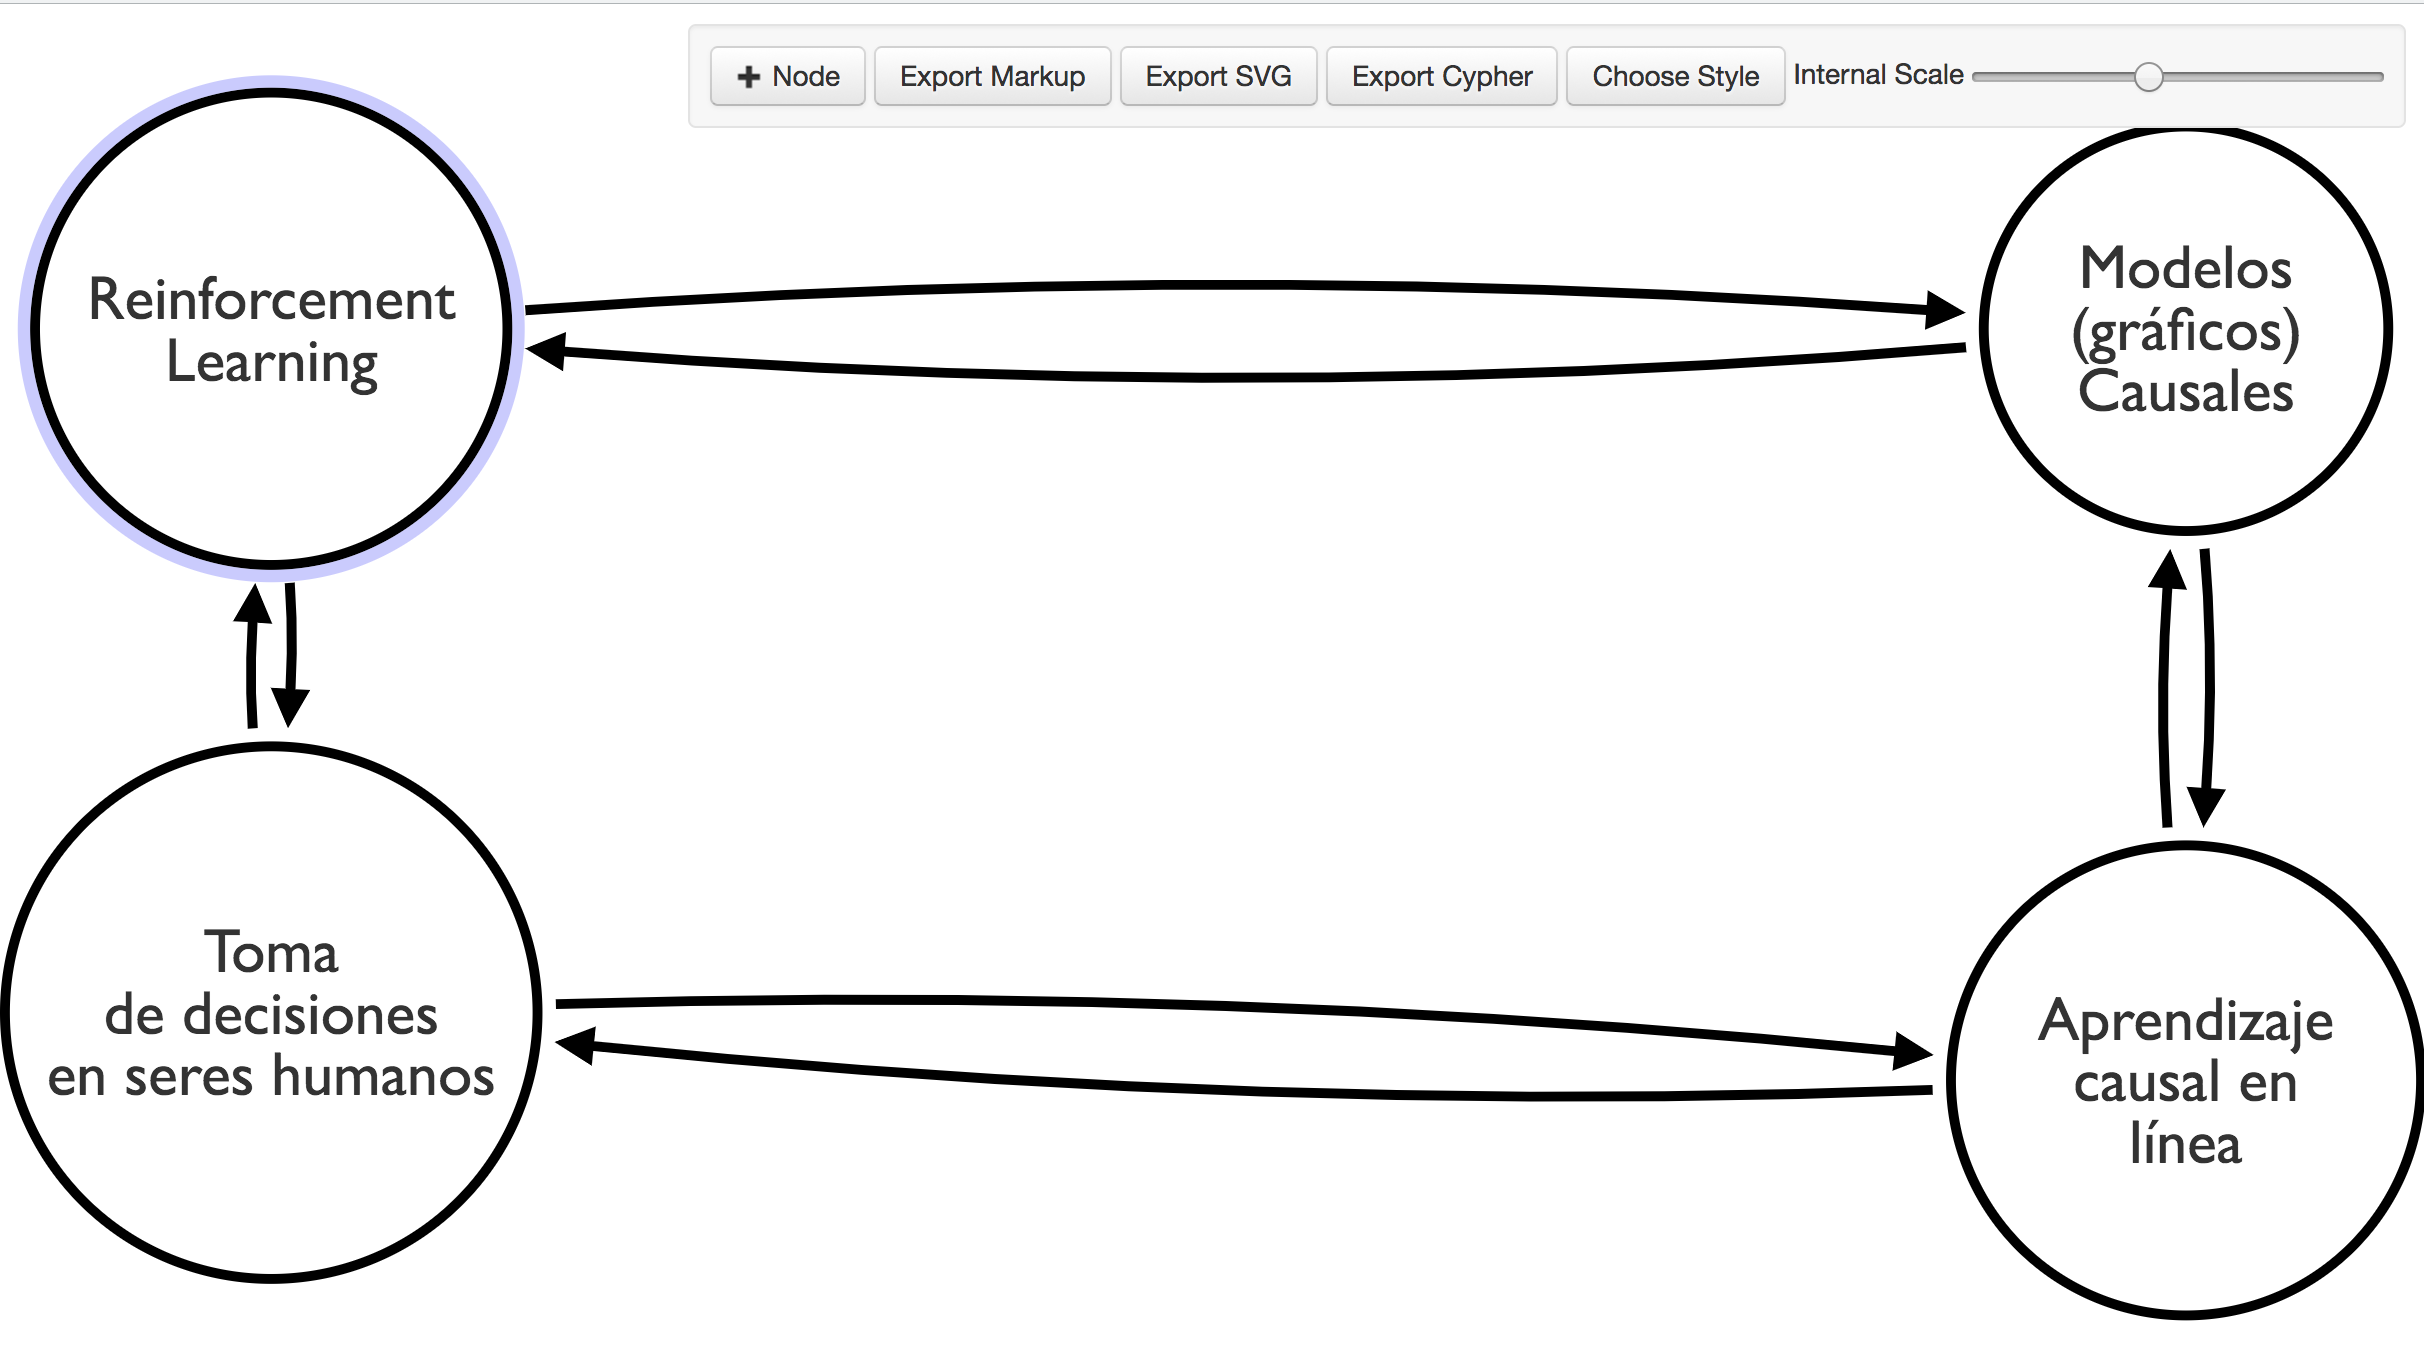
\includegraphics[scale=0.3]{/Users/MauricioGS1/INAOE/Primer_Semestre/Figures/diagrama.png}
\end{center}
\subsection{Pasos a seguir}
\begin{itemize}
\item ¿Por qué esto sería mejor que trabajo de Garnelo?
\item Tengo un modelo causal \textit{verdadero}, ¿cómo lo incorporo en una política de RL? ¿cómo guío el descubrimiento de acciones? Aquí ayuda el artículo de \cite{lattimoreNIPS2016}
\item Tengo una política aprendida, ¿cómo descubro estructura causal? Aquí puede ayudar el artículo de \cite{ortega2014generalized}
\item ¿Qué aprendo primero?
\item ¿Cómo le doy más peso a la información explicativa que a la información reactiva?
\item Exploración vs explotación causal: ¿cómo decido si seguir la info causal o tomar acciones exploratorias para descubrir relaciones causales? 
\item ¿Un dominio de interés? 
\end{itemize}
\subsection{Ejemplo: Caso de un MDP finito}
En el caso de un MDP finito completamente especificado; es decir, en el cual conocemos las probabilidades de transición y las recompensas. Un modelo causal sobre este dominio opera sobre las acciones, pues son estas las que \textbf{\textit{suponemos}} que \textit{causan} algo; esto es, 
\[ a \xrightarrow[]{\text{causa}} \textrm{estado del mundo}. \]
Entonces, en un modelo gráfico causal necesitaremos tener \textit{nodos de estado}, así como \textit{nodos de acciones} (\textit{causal decision graphs}).\\
\\
Es claro que los estados del mundo afectarán la siguiente decisión, pero no causan nada por sí mismos; en todo caso, el estado afeca la decisión pero sólo a través de la política (el valor del estado).\\
\\
El objetivo, ahora, es aprender una política que incorpore conocimiento causal, el cual a su vez fue aprendido mediante interacción.\\
\\
Suponiendo que conocieramos el modelo causal, entonces este nos ayudará a escoger acciones. Ya no debería usar políticas $\varepsilon$-greedy para explorar el espacio, pues ya conozco relaciones útiles. El enfoque de \cite{lattimore2017nips} podría servir aquí.
\\
Por otro lado, cómo ir estimando la estructura causal del grafo? Parece ser que la estadística Bayesiana es una idea, pues en cada pasao tengo creencias sobre la estructura causal que voy a modificar a la luz de la evidencia, la evidencia está dada por los descubrimientos del agente y las creencias por la estructura actual del grafo.
\\
¿El valor de un estado debe cambiar en el caso causal? Para que el valor de un estado se vea afectado por lo que pueda causar el agente a partir de ese estado se necesita algún tipo de función de utilidad, ¿no? No lo sé...
\newpage
\bibliographystyle{apalike}
\bibliography{Bibliografia}
\appendix
\section{Teoría de Probabilidad}
\section{Estadística Bayesiana}

\end{document}